%%%%%%%%%%%%%%%%%%%%%%%%%%%%%%%%%%%%%%%%%
%  Telemac Documentation
%  Example of the TelemacDoc class
%
%%%%%%%%%%%%%%%%%%%%%%%%%%%%%%%%%%%%%%%%%

%----------------------------------------------------------------------------------------
%	PACKAGES AND OTHER DOCUMENT CONFIGURATIONS
%----------------------------------------------------------------------------------------
\documentclass[Courlis]{../../data/TelemacDoc} % Default font size and left-justified equations
%\documentclass[Courlis,french]{TelemacDoc} % Default font size and left-justified equations in french

%%---------------------------------------------------------------------------
%% Command for COURLIS names
%%---------------------------------------------------------------------------
\newcommand{\Cbedload}{{\scshape Courlis-bedload}\xspace}
\newcommand{\Csuspension}{{\scshape Courlis-suspension}\xspace}
\newcommand{\fudaa}{{\scshape Fudaa-Mascaret}\xspace}
\newcommand{\precourlis}{{\scshape PreCourlis}\xspace}
\newcommand{\cas}{\telfile{cas file}\xspace}
\newcommand{\cass}{\telfile{cas files}\xspace}
\newcommand{\xcas}{\telfile{xcas file}\xspace}
\newcommand{\xcass}{\telfile{xcas files}\xspace}
%%---------------------------------------------------------------------------
%% Nomenclature
%%---------------------------------------------------------------------------
\usepackage{ifthen}
\usepackage{nomencl}
%
\makenomenclature
\renewcommand{\nompreamble}{\markboth{%
                            \MakeUppercase\nomname}{\MakeUppercase\nomname}%
                           }
\newcommand{\nomunit}[1]{%
\renewcommand{\nomentryend}{\hspace*{\fill}#1}}
% \usepackage{subcaption} % Not compatible with subfig
\definecolor{codegreen}{rgb}{0,0.6,0}
\definecolor{codegray}{rgb}{0.5,0.5,0.5}
\definecolor{codepurple}{rgb}{0.58,0,0.82}
\definecolor{backcolour}{rgb}{0.95,0.95,0.92}

\lstdefinestyle{mystyle}{
    backgroundcolor=\color{backcolour},
    commentstyle=\color{codegreen},
    keywordstyle=\color{magenta},
    numberstyle=\tiny\color{codegray},
    stringstyle=\color{codepurple},
    basicstyle=\ttfamily\scriptsize,
    breakatwhitespace=false,
    breaklines=true,
    captionpos=b,
    keepspaces=true,
    numbers=left,
    numbersep=5pt,
    showspaces=false,
    showstringspaces=false,
    showtabs=false,
    tabsize=2
}

\lstset{style=mystyle}

\lstdefinelanguage{TelemacCasRed}{
  basicstyle=\ttfamily\footnotesize,
  commentstyle=\color{PantoneRed},
  morecomment=[f]{/},
}
%----------------------------------------------------------------------------------------

\begin{document}

\let\cleardoublepage\clearpage

%----------------------------------------------------------------------------------------
%	TITLE PAGE
%----------------------------------------------------------------------------------------
\title{\courlis}
\subtitle{User Manual}
\version{\telmaversion}
\date{\today}
\maketitle
\clearpage


%----------------------------------------------------------------------------------------
%	COPYRIGHT PAGE
%----------------------------------------------------------------------------------------

\newpage

\thispagestyle{empty}

\TelemacCopyright{}


%----------------------------------------------------------------------------------------
%	TABLE OF CONTENTS
%----------------------------------------------------------------------------------------


\pagestyle{empty} % No headers

\tableofcontents% Print the table of contents itself

%\cleardoublepage % Forces the first chapter to start on an odd page so it's on the right

\pagestyle{fancy} % Print headers again

\printnomenclature

%----------------------------------------------------------------------------------------
%	Introduction
%----------------------------------------------------------------------------------------
\addcontentsline{toc}{section}{Introduction}
\chapter*{Introduction}\label{intro}
\chapter{Introduction}

\waqtel (WAter Quality for TELemac) is a component of the Telemac-Mascaret system (TMS)
which focuses on the water quality aspects.
It was developped to allow the TMS's users to tackle water quality problems
together with hydrodynamics.

Up to release V7P0, \telemac{2D} and \telemac{3D} were coupled with DELWAQ,
the Deltares water quality code.
This coupling, though working well for simple and medium sized models,
was not suitable and cumbersome for big models.
The main issue related to the use of \telemac-DELWAQ was
the uncompatible parallelization of both codes.

To overcome this issue and in order to fully benefit
from the parallelization efficiency of the TMS, the development team
introduced a first version of \waqtel in the V7P1 release. 

\waqtel is developed by the LNHE (Laboratoire National d'Hydraulique et
Environnement) of the Research and Development Division of EDF (EDF-R\&D). As
for previous versions, the 7.1 release of the code complies with the Quality
Assurance procedures of scientific and technical softwares of EDF-R\&D. It is a
process of construction and verification of the product quality in the
different phases of his life. In particular, a software following the Quality
Assurance procedures comes with a Validation Folder that describes the intended
use of the software and a set of test cases. This document allows you to judge
the performance and limitations of the software, situating the field of
application. These tests are also used in the development of the software and are
checked at every new release.

\section{Position of the \waqtel code within the telemac modelling system}

The \waqtel software is part of the TELEMAC modelling system developed by
the LNHE of EDF R\&D. TELEMAC is a set of modelling tools allowing to treat
every aspects of natural free surface hydraulics: currents, waves, transport of
tracers and sedimentology.
\newline
\waqtel, unlike other compnents of the TMS, can not be run in a stand-alone mode.
To run a \waqtel model, it is necessary to run \telemac{2D} or \telemac{3D} coupled 
with \waqtel using the keyword \telkey{COUPLING WITH} = 'WAQTEL'
(in French: \telkey{COUPLAGE AVEC} ='WAQTEL').

The pre-processing and post-processing of simulations can be done either
directly within the TELEMAC system or with different software that present an
interface of communication with the system. We can particularly mention the
following tools:

\begin{itemize}
\item the FUDAA-PREPRO software, developed from the FUDAA platform
by the CEREMA's Recherche, Informatique et Modélisation Department, covers all
the pre-processing tasks involved by the achievement of a numerical hydraulic
study, as well as a graphical post-processing tool,
\item the Blue Kenue software, developed the Hydraulic Canadian
Center, proposes a powerful mesh generation tool and a user-friendly
post-processing tool,
\item the Janet software, developed by Smile Consult GmbH, which offers among
others, a mesh generation tool,
\item the ParaView software, developed by Sandia National Laboratories, Los
Alamos National Laboratory and Kitware, which enables to visualise 3D results,
big data in particular and is open source,
\item the SALOME-HYDRO software based on the SALOME platform, developed by EDF,
CEA and OPENCASCADE which enables to handle raw data (bathymetry, maps,
pictures, LIDAR\ldots) until the mesh generation.
The post-processing tool ParaViS available in the SALOME platform is based on
the ParaView software and can visualise 1D, 2D or 3D results.
A first version of SALOME-HYDRO has been available since Spring 2016,
\item the QGIS software, which is an open source Geographic Information System.
\end{itemize}


\section{Software environment}

All the simulation modules are written in FORTRAN 90, with no use of the
specific language extensions in a given machine. They can be run on all the PCs
(or PC "clusters") under Windows and Linux operating systems as well as on the
workstations under the Unix operating system.

\section{User programming}

When using a simulation module from the TELEMAC system, the user may have to
program specific subroutines which are not in the code's standard release. In
particular, that is made through a number of so-called «~user~» subroutines.
These subroutines are written so that they can be modified, provided that the
user has a basic knowledge in FORTRAN language, with the help of the «~Guide
for programming in the Telemac system~» \cite{HervouetProg2009}.

The procedure to be carried out in that case comprises the steps of:

\begin{itemize}
\item recovering the standard version of the user subroutine(s) as supplied in
the distribution and copying it into the current directory,
\item amending the subroutine(s) according to the model to be constructed,
\item concatenating the whole set of subroutines into a single FORTRAN file
which will be compiled during the \telemac{2D} or \telemac{3D} launching process.
\end{itemize}

During that programming stage, the user can gain access to the various
variables of the software through the FORTRAN 90 structures.

All the data structures are gathered within FORTRAN files, which are known as
modules. For \waqtel, the file name is \telfile{DECLARATION\_WAQTEL.f}. To gain
access to the \waqtel data, just insert the command \telfile{USE
DECLARATIONS\_WAQTEL} into the beginning of the subroutine. Adding the
command \telfile{USE BIEF} may also be necessary in order to reach the structure in the
\bief library.

Nearly all the arrays which are used by \waqtel are declared in the form of
a structure. For example, the access to the water depth array will be in the
form \telfile{H\%R}, \telfile{\%R} meaning it is a real-typed pointer.
In case of an integer-typed pointer, the \telfile{\%R} is replaced by a \telfile{\%I}.
However, in order to avoid having to handle too many \telfile{\%R} and \telfile{\%I},
a number of aliases are defined, such as, the \telfile{NPOIN3}, \telfile{NELEM3} and
\telfile{NPTFR2} variables. For further details, the user can refer to
the programming guide in TELEMAC \cite{HervouetProg2009}.

\newpage
%----------------------------------------------------------------------------------------
%	CHAPTER 1: Theoretical aspects
%----------------------------------------------------------------------------------------
\chapter{Theoretical aspects}\label{chap1}
\section{Hydrodynamics}
\mascaret solves the shallow water equations for incompressible flow, hydrostatic pressure and uniform distribution of velocities along the vertical axis. The flow slope and the horizontal curvature radius are supposed low. Wind effects on the free surface are also neglected. Flow is described on each section through mean velocity and mean free surface elevation.

\begin{CommentBlock}{Limit} 
	To use \courlis, only one reach can be considered. Besides, only the main channel can be taken into account and no singularities can be modeled.
\end{CommentBlock}

%%%%%%%%% ST VENANT %%%%%%%%%
\subsection{Shallow water equations}
The shallow water equations with variable section are given below :
\bequ
    \left\{
        \begin{array}{ll}
            \frac{\partial S}{\partial t} + \frac{\partial Q}{\partial x} = q_l\\
            \frac{\partial Q}{\partial t} + \frac{\partial \beta \frac{Q^2}{S}}{\partial x} + gZ\left( \frac{\partial Z}{\partial x} +J\right)= \frac{Q}{S} q_l\\
        \end{array}
    \right.
    \label{eq:shallow}
\eequ

with :
\begin{itemize}
	\item $S$ the wetted area ;
	\item $q_l$ the lateral inflows (confluence) in $m^2.s^{-1}$ ;
	\item $Q$ the mean discharge across the section ;
	\item $Z$ the free surface elevation ;
	\item $g$ the acceleration due to gravity ;
	\item $J$ the mean energy dissipation rate ;
	\item $\beta$ accounts for the variations of the real flow velocity accross the section \cite{mascaret_guide}.
\end{itemize}

\nomenclature{$S$}{Wetted area \nomunit{$m^2$}}
\nomenclature{$t$}{Time \nomunit{$s$}}
\nomenclature{$x$}{Longitudinal space variable \nomunit{$m$}}
\nomenclature{$q_l$}{Lateral inflows \nomunit{$m^2.s^{-1}$}}
\nomenclature{$g$}{Gravity acceleration \nomunit{$m^2.s^{-1}$}}
\nomenclature{$Q$}{Mean discharge accross the section \nomunit{$m^3.s^{-1}$}}
\nomenclature{$Z$}{Mean free surface elevation across the section \nomunit{$m$}}
\nomenclature{$J$}{Mean energy dissipation rate or energy slope \nomunit{$m.m^{-1}$}}

%%%%%%%%% RUGOSITE %%%%%%%%%
\subsection{Friction}
Bed and shores shear stress is taken into account through the Strickler friction law :
\bequ
	J = \frac{Q^2}{S^2 K^2 R_h^{\frac{4}{3}}}
	\label{eq:strickler}
\eequ
where :
\begin{itemize}
	\item $K$ is the Strickler coefficient ;
	\item $R_h$ the hydraulic radius.
\end{itemize}

The local shear stress $\tau_{tot}$ is computed by :

\bequ
	\tau_{tot} = \rho_w g R_h J = \frac{\rho_w g U^2}{K^2 R_h^{\frac{1}{3}}}
	\label{eq:contrainte_totale}
\eequ
For real cases, the hydraulic radius is usually approximated by the mean water depth across the section : $R_h \sim H$.
This option is activated by default in \courlis. 

\nomenclature{$H$}{Mean water depth across the section \nomunit{$m$}}
\nomenclature{$K$}{Strickler coefficient \nomunit{$m^{\frac{1}{3}}.s^{-1}$}}
\nomenclature{$R_h$}{Hydraulic radius \nomunit{$m$}}

%%%%%%%%% PLANIMETRAGE %%%%%%%%%
\subsection{Vertical discretization}
\label{planim}

Vertical discretization is used to transform cross-sections (2D) to unidimensional variables. Curves are generated for each section to link hydraulic radius, discharges, wetted areas, wetted perimeters and widths at the free surface to the elevation (starting at the lowest point of the section with a spatial step chosen by the user as shown on the Figure \ref{fig:planimetrage} below). 

\begin{figure}[htb!]
    \centering
    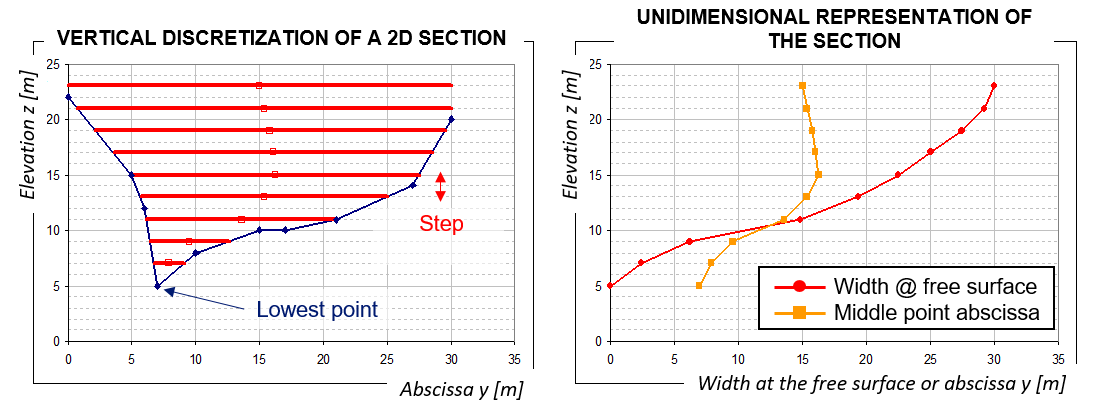
\includegraphics[width=\textwidth]{./graphics/planimetrage.png}
    \caption{Vertical discretization of a section : for each elevation, the width at the free surface and the middle point abscissa of the free surface are computed}
    \label{fig:planimetrage}
\end{figure}

For long-term simulations with a lot of bed evolutions, vertical discretization becomes time-consuming et can represent on its own up to more than 90\% of the total calculation time \cite{thesis_ung}. Clipping parameters can reduce the calls to the vertical discretization process. 

%%%%%%%%% TRANSPORT SOLIDE %%%%%%%%%
\section{Sediment transport}
\label{sediment_transport_th}
\courlis development was initiated in 1990 by EDF to model fine particles transport for the emptying of the Grangent reservoir in 1995. The bedload module of \courlis has been maintained and developed since 2012 and the Hydraulic Engineering Centre of EDF is officialy in charge of this module inside EDF since 2015.

The two modules can not be used simultaneously so no sediment mixing can be modeled with \courlis.

Up to 6 sediment layers (i.e. 7 interfaces) can be modeled in \courlis. Sediment interfaces are described in the geoC file (cf \S \ref{geoC_file}) and define homogeneous layers of sediment such as a 100$\%$ sand layer, a 100$\%$ silt layer and a mixed silt-sand sediment layer with the suspension module or a gravel layer and a bottom layer with the bedload module for example. Their elevation, and thus the width of the sediment layers, can vary transversaly as shown on Figure \ref{fig:layers} below.

\begin{figure}[htb!]
   \begin{minipage}[c]{.48\linewidth}
	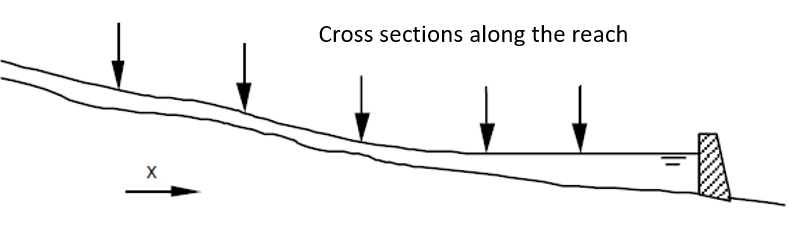
\includegraphics[width=\textwidth]{./graphics/Plong.png} 
	\caption{Longitudinal profile of a reach}
	\label{fig:PLong}
   \end{minipage} \hfill
   \begin{minipage}[c]{.48\linewidth}
	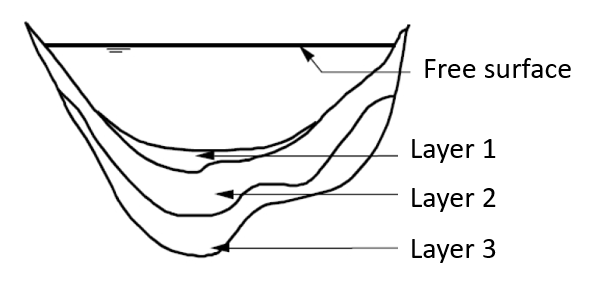
\includegraphics[width=\textwidth]{./graphics/layers.png} 
	\caption{Cross-section view of sediment layers in \courlis}
	\label{fig:layers}
   \end{minipage}
\end{figure}

%\begin{figure}[htb!]
%    \centering
%    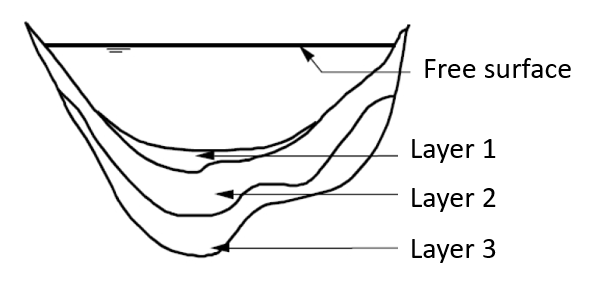
\includegraphics[width=0.7\textwidth]{./graphics/layers.png}
%    \caption{Sediment layers in \courlis}
%    \label{fig:layers}
%\end{figure}

The local shear stress can be decomposed into a stress associated to the skin friction, also called efficient shear stress, $\tau_{eff}$ and a stress due to bed forms $\tau_{forms}$ : 
$\tau_{tot} = \tau_{eff} + \tau_{forms} $
The skin friction coefficient is often computed from grain sizes, for example with the Strickler formula (Equation \ref{eq:strickler_kp}) or the Meyer-Peter and Müller formula (Equation \ref{eq:MPM_kp}).

\bequ
	K_p = \frac{21}{d_{50}}^\frac{1}{6}
	\label{eq:strickler_kp}
\eequ

\bequ
	K_p = \frac{26}{d_{90}}^\frac{1}{6}
	\label{eq:MPM_kp}
\eequ
$d_{50}$ is the median grain diameter and $d_{90}$ is the diameter for which 90\% of the grains are smaller.

\begin{WarningBlock}{Warning}
	For really fine sediment (< 200 $\mu m$ and cohesive sediment), these formulae become irrelevant and would give surfaces too smooth for natural beds. 
	In practice, skin friction should be limited to a maximal value of 85.
	This is the case when looking for deposition and erosion conditions for cohesive sediment ; a critical shear stress value of 85 Pa is systematically used.
\end{WarningBlock}

The efficient shear stress is estimated as 
\bequ
	\tau_{eff} = \tau_{tot} \left( \frac{K}{K_p} \right)^\gamma
\eequ  
with $\gamma$ a coefficient, by default equal to 2.

The Shields number $\theta$ is defined as :
\bequ
	\theta = \frac{\tau_{tot}}{(\rho_s-\rho_w) g d_{50}}
\eequ

Using Equation \ref{eq:contrainte_totale}, this expression becomes :
\bequ
	\theta = \frac{U^2}{R K^2 R_h^{\frac{1}{3}} d_{50}}
	\label{eq:shields}
\eequ
 $R$ is the relative reduced density $R=\frac{\rho_s}{\rho_w}-1 = s - 1$.

%%%%%%%%%%%%%%%%%%%%%%% SUSPENSION %%%%%%%%%%%%%%%%%%%%%%%
\subsection{\Csuspension}
Sediment in \Csuspension are considered as a passive tracer (no influence on the hydrodynamics), hence the fluid is always considered as a Newtonian fluid. 
The conservative form of the advection-diffusion equation for suspended sediment transport transport links the averaged concentration $C$ of the sediment with the erosion and deposition source terms $E$ and $D$.

\bequ
    \frac{\partial SC}{\partial t} + \frac{\partial QC }{\partial x}=\frac{\partial}{\partial x} \left (k_x S \frac{\partial C}{\partial x} \right) + E - D + q_{confluence}
\eequ

\begin{itemize}
	\item $k_x$ is the longitudinal dispersion coefficient ;
	\item $q_{confluence}$ the local inflows at a confluence for example.
\end{itemize}
The longitudinal dispersion coefficient can be estimated from \cite{Kas02} as done in \cite{Hau14}. 

Cohesive and non-cohesive sediment transport are supposed independant.

%%%%%%%%% VASE %%%%%%%%%
\subsubsection{Cohesive sediment fluxes}
%\tau_{tot} = \frac{\rho g H U^2}{K_p^2 R_h^{\frac{4}{3}}} ???
Cohesive sediment transport is considered unsaturated, i.e. concentration in the fluid is not limited (no saturation effect).
Deposition flux for cohesive sediment is computed with the empirical Krone law \cite{krone}.
\bequ
    \label{eq:krone}
    D = \left\{
        \begin{array}{ll}
            w_s C \left(1- \frac{\tau}{\tau_{c, deposition}}\right) \  \textrm{if}\  \tau < \tau_{c, deposition} , \\
            0 \  \textrm{otherwise}\\
        \end{array}
    \right.
\eequ
where $\tau$ is the bed shear stress, $\tau_{cr, deposition}$ the critical bed shear stress for deposition and $w_s$ the settling velocity for silts. 
 
Similarly, erosion flux is computed with the empirical Partheniades law \cite{partheniades} :

\bequ
    \label{eq:parth}
    E = \left\{
        \begin{array}{ll}
            M \left(\frac{\tau}{\tau_{c, erosion}} - 1 \right)  \  \textrm{if}\  \tau > \tau_{c, erosion} , \\
            0 \  \textrm{otherwise}\\
        \end{array}
    \right.
\eequ
where $\tau_{cr, erosion}$ is the critical bed shear stress for erosion and $M$ the Partheniades constant.
\begin{WarningBlock}{Note}
	For cohesive sediment, the critical bed shear stress $\tau_{cr}$ may be different for deposition and erosion, i.e. there can be a range of bed shear stresses for which there is no deposition or erosion (suspended load). 
	This is not the case for non-cohesive sediment. 
\end{WarningBlock}

%%%%%%%%% SAND %%%%%%%%%
\subsubsection{Non-cohesive sediment fluxes}
Sand transport is supposed saturated and is estimated via the Engelund-Hansen formula \cite{engelund}.
This formula is valid for grain sizes between 0.15 mm and 0.9 mm ($d_{50}$) and low slopes. 

\bequ
    \label{eq:engelund}
    q_s = 0.05 \sqrt{\frac{Rd_{50}^3}{g}} K^2 R_h^{\frac{1}{3}} \theta^{\frac{5}{2}}
\eequ
with $\theta$ the Shields number defined in Equation \ref{eq:shields}.

An equilibrium concentration is then defined as $C_{eq}=\frac{q_s \rho_s}{Q}$. 
When the solid discharge becomes higher than the transport capacity $C > C_{eq}$, the sediment flux becomes a deposition flux. Similarly, when the solid discharge is lower than the transport capacity $C < C_{eq}$, the flux becomes an erosion flux as described in the following equation :
\bequ
    q_s = \left\{
        \begin{array}{ll}
            \alpha w_s (C_{eq} - C)  \  \textrm{if}\  C > C_{eq} , \\
            \alpha w_s (C - C_{eq})  \  \textrm{otherwise}\\
        \end{array}
    \right.
\eequ
where $\alpha$ is an adjustment coefficient to the new equilibrium for suspension \cite{Che10}. 
It represents the velocity with which the sediment system tends to its new equilibrium state.
The sand settling velocity $w_s$ can be estimated thanks to the Stokes law (1851) or the Camenen formula \cite{Cam04}.


\nomenclature{$\alpha$}{Adjustment coefficient to the new equilibrium for suspension \nomunit{$\emptyset$}}

\nomenclature{$C$}{Suspended sediment concentration \nomunit{$g.L^{-1}$}}
\nomenclature{$I_f$}{Bottom slope \nomunit{$m/m$}}
\nomenclature{$I_{solid\ inflows}$}{Equilibrium slope for solid inflows \nomunit{$m/m$}}
\nomenclature{$k_x$}{Longitudinal dispersion coefficient along the $x$ axis \nomunit{$m^2.s^{-1}$}}
\nomenclature{$w_s$}{Settling velocity \nomunit{$m.s^{-1}$}}
\nomenclature{M}{Partheniades constant \nomunit{$kg.m^{-2}.s^{-1}$}}

%%%%%%%%% EVOLUTION DES FONDS %%%%%%%%%
\subsubsection{Bed evolution}

The bed evolution of the layer i during $\Delta t$ is computed with the solid discharges of deposition and erosion of the different layers :
\bequ
    \Delta h_{i, deposition}(\Delta t) = \frac{q_{deposition}\Delta t}{C_i}
\eequ

\bequ
    \Delta h_{i, erosion}(\Delta t)  = -\left(\sum h_{k, (\Delta t - \Delta t_1)} + \frac{q_{erosion}\Delta t_1 }{C_{i}}\right)
\eequ

where the variation in height of the layer $i$ by deposition or erosion is noted $\Delta h_i$ end the height of the layer $k$ eroded between $\Delta t_1$ and $\Delta t$ is noted $h_{k, (\Delta t - \Delta t_1)}$.

\nomenclature{$\Delta h_i$}{Height evolution of the sediment layer $i$ by deposition or erosion \nomunit{$m$}}
\nomenclature{$h_{i, \Delta t - \Delta t_1}$}{Height of the sediment layer $i$ eroded between $\Delta t_1$ and $\Delta t$ \nomunit{$m$}}

%%%%%%%%%%%%%%%%%%%%%%% BEDLOAD %%%%%%%%%%%%%%%%%%%%%%%
\subsection{\Cbedload}
For now, only one grain size distribution can be given to \Cbedload for all layers and all sections. 
\Cbedload is therefore commonly used with only one sediment layer i.e. two interfaces (one interface between the movable gravel bed and the water and a second one to separate the gravel bed from immovable non-erodible materials).
 
%%%%%%%%% EXNER %%%%%%%%%
\subsubsection{Bed evolution}
 This module is based on the Exner continuity equation (\ref{eq:exner}) to model gravel transport and bed evolutions in rivers or reservoirs. It does not take into account armoring and paving phenomena.

\bequ
     \rho_S (1-\rho) \frac{\partial Z_b}{\partial t} + \frac{\partial Q_s}{\partial x} = 0 
     \label{eq:exner}
\eequ

Resolution is done thanks to a finite volume scheme. The numerical flux term between two cells is computed with an uncentered scheme depending on the flow regime \cite{thesis_ung} : 

\begin{figure}[H]
	\centering
	\subfloat[Subcritical input -- Subcritical output]{
			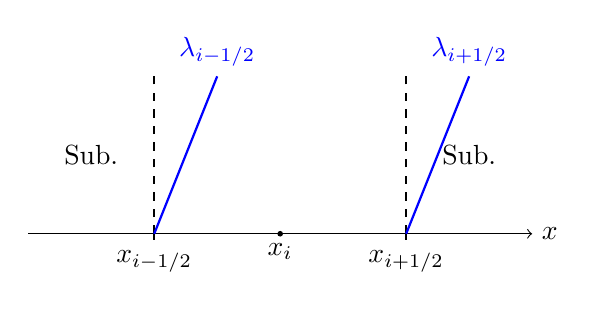
\begin{tikzpicture}[scale=0.4]
			  \draw[->]         (-8,0) -- (8,0)   node[right] {$x$};
			  \draw[thick,dashed]  (-4,0) -- (-4,5.);
			  \draw[thick,dashed] (4,0) -- (4,5.)  node[above] {};

			  \draw[thick] (-4,0.2)--(-4,-0.2) node[below] {$x_{i-1/2}$};
			  \draw[thick] (4,0.2)--(4,-0.2) node[below] {$x_{i+1/2}$};
			  \draw[fill=black] (0,0) circle (2pt) node[below]{$x_{i}$};

			  \draw (-6,2.5) node {Sub.};
			  \draw (6,2.5) node {Sub.};
			  \draw[color=blue, thick]  (-4,0) -- (-2,5)   node[above] {$\lambda_{i-1/2}$};
			  \draw[color=blue, thick]  (4,0) -- (6,5)     node[above] {$\lambda_{i+1/2}$};
			\end{tikzpicture}
	\label{fluvin_fluvout}
	}
	\hfill
	\subfloat[Supercritical input -- Supercritical output]{
		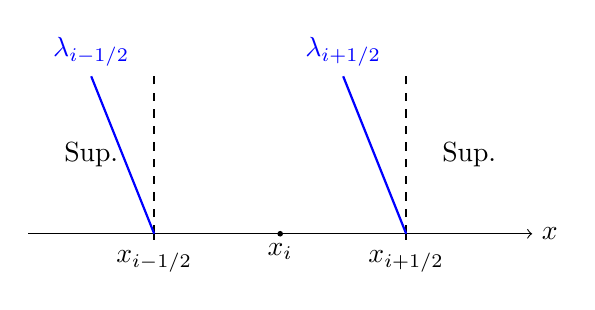
\begin{tikzpicture}[scale=0.4]
		  \draw[->]         (-8,0) -- (8,0)   node[right] {$x$};
		  \draw[thick,dashed]  (-4,0) -- (-4,5.);
		  \draw[thick,dashed] (4,0) -- (4,5.)  node[above] {};

		  \draw[thick] (-4,0.2)--(-4,-0.2) node[below] {$x_{i-1/2}$};
		  \draw[thick] (4,0.2)--(4,-0.2) node[below] {$x_{i+1/2}$};
		  \draw[fill=black] (0,0) circle (2pt) node[below]{$x_{i}$};

		  \draw (-6,2.5) node {Sup.};
		  \draw (6,2.5) node {Sup.};
		  \draw[color=blue, thick]  (-4,0) -- (-6,5)   node[above] {$\lambda_{i-1/2}$};
		  \draw[color=blue, thick]  (4,0) -- (2,5)     node[above] {$\lambda_{i+1/2}$};
		\end{tikzpicture}
		\label{torin_torout}
	}

	\subfloat[Subcritical input -- Supercritical output]{
		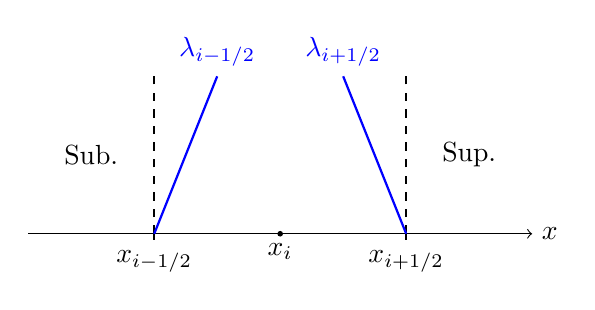
\begin{tikzpicture}[scale=0.4]
		  \draw[->]         (-8,0) -- (8,0)   node[right] {$x$};
		  \draw[thick,dashed]  (-4,0) -- (-4,5.);
		  \draw[thick,dashed] (4,0) -- (4,5.)  node[above] {};

		  \draw[thick] (-4,0.2)--(-4,-0.2) node[below] {$x_{i-1/2}$};
		  \draw[thick] (4,0.2)--(4,-0.2) node[below] {$x_{i+1/2}$};
		  \draw[fill=black] (0,0) circle (2pt) node[below]{$x_{i}$};

		  \draw (-6,2.5) node {Sub.};
		  \draw (6,2.5) node {Sup.};
		  \draw[color=blue, thick]  (-4,0) -- (-2,5)   node[above] {$\lambda_{i-1/2}$};
		  \draw[color=blue, thick]  (4,0) -- (2,5)     node[above] {$\lambda_{i+1/2}$};
		\end{tikzpicture}
		\label{fluvin_torout}
	}
	\hfill
	\subfloat[Supercritical input -- Subcritical output]{
		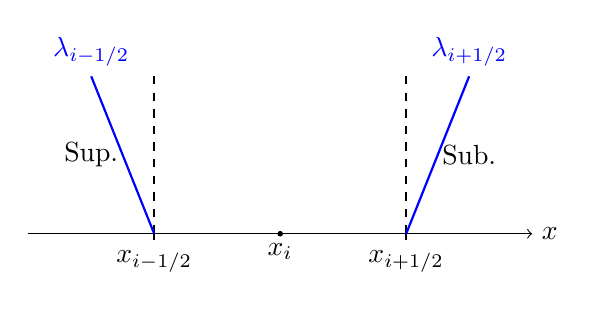
\begin{tikzpicture}[scale=0.4]
		  \draw[->]         (-8,0) -- (8,0)   node[right] {$x$};
		  \draw[thick,dashed]  (-4,0) -- (-4,5.);
		  \draw[thick,dashed] (4,0) -- (4,5.)  node[above] {};

		  \draw[thick] (-4,0.2)--(-4,-0.2) node[below] {$x_{i-1/2}$};
		  \draw[thick] (4,0.2)--(4,-0.2) node[below] {$x_{i+1/2}$};
		  \draw[fill=black] (0,0) circle (2pt) node[below]{$x_{i}$};

		  \draw (-6,2.5) node {Sup.};
		  \draw (6,2.5) node {Sub.};
		  \draw[color=blue, thick]  (-4,0) -- (-6,5)   node[above] {$\lambda_{i-1/2}$};
		  \draw[color=blue, thick]  (4,0) -- (6,5)     node[above] {$\lambda_{i+1/2}$};
		\end{tikzpicture}
		\label{torin_fluvout}
		}
	
	\caption{Different situations depending on the nature of the flow at the input and output of a cell from \cite{thesis_ung} - $\lambda$ is the wave velocity associated to the bed evolution.}
	\label{fig:allregcell}
\end{figure}

\nomenclature{$\lambda_i$}{Wave velocity associated to bed evolution in cell $i$ \nomunit{$m.s^{-1}$}}

Depending on the flow motion at the input and the output of the cell $i$, the variation of volume in the cell $i$ between two consecutive timsteps is computed from the following finite volume scheme :

\bequ
\begin{gathered}\label{eq:exner-scheme}
{(V)_i^{n+1} - (V)_i^n =}\\
\left\{
        \begin{array}{ll}
		  -\frac{\delta t}{\delta x} \left( (Q_s)_{i+1}^n - (Q_s)_{i}^n \right) & \textrm{if} \  (F_r)_{i-1/2} < 1 \  \textrm{and} \  (F_r)_{i+1/2} < 1 \  \textrm{(case \ref{fluvin_fluvout}),} \\
		  -\frac{\delta t}{\delta x} \left( (Q_s)_{i}^n - (Q_s)_{i-1}^n \right) & \textrm{if} \ (F_r)_{i-1/2} > 1 \  \textrm{and} \ (F_r)_{i+1/2} > 1 \  \textrm{(case \ref{torin_torout}),} \\
		  -\frac{\delta t}{2 \delta x} \left( (Q_s)_{i+1}^n - (Q_s)_{i-1}^n \right) & \textrm{if} \  (F_r)_{i-1/2} < 1 \  \textrm{and} \ (F_r)_{i+1/2} > 1 \  \textrm{(case \ref{fluvin_torout}),} \\
  0 & \textrm{if} \  (F_r)_{i-1/2} > 1 \  \textrm{and} \  (F_r)_{i+1/2} < 1 \  \textrm{(case \ref{torin_fluvout}).}
	\end{array}
	\right.
\end{gathered}
\eequ
where 
\begin{itemize}
	\item $(V)_i^n$ is the volume of sediment in the cell $i$ at the timestep $n$ ;
	\item $\delta t$ is the timestep ;
	\item $\delta x$ is the spacestep ;
	\item $(Q_s)_{i}^n$ is the solid discharge in the cell $i$ at the timestep $n$ given by the transport law ;
	\item $F_r$ is the Froude number defined such as \[ F_r = \dfrac{u}{\sqrt{gh_w}} \] with $h_w$ the water depth. 
\end{itemize}

\nomenclature{$h_w$}{Water depth \nomunit{$m$}}
\nomenclature{$F_r$}{Froude number \nomunit{$\emptyset$}}
\nomenclature{$V_i^n$ }{Volume of sediment in cell $i$ at the timestep $n$ \nomunit{$m^{3}$}}

The bottom elevation is then updated accordingly to the variation of volume computed above. The solid discharge $(Q_s)_{i}^n$ in cell $i$ at the timstep $n$ is computed with different transport formulae described below. 

\nomenclature{$Z_b$}{Bottom elevation \nomunit{$m$}}

Evolution of the river bottom is not applied in the same way for erosion and for deposition :
\begin{itemize}
 \item Evolution due to erosion is applied uniformely on all points of the river bottom located under the free surface ;
 \item Evolution due to deposition is applied horizontally (at constant elevation). For each horizontal deposition surface, the corresponding elevation is computed by linear interpolation of the curves generated by vertical discretization (cf Section \ref{planim}).
\end{itemize}

\begin{figure}[htb!]
    \centering
    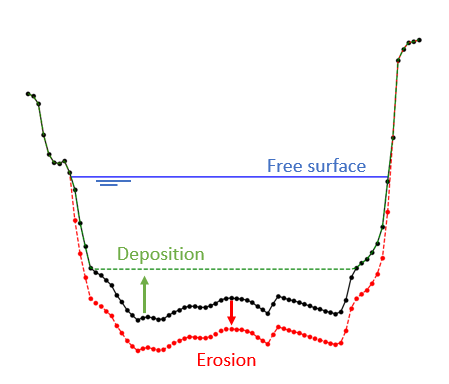
\includegraphics[width=0.45\textwidth]{./graphics/erosion_deposition.png}
    \caption{Deposition and erosion mechanisms in \Cbedload}
    \label{fig:depo_ero}
\end{figure}

%%%%%%%%% FORMULES DE TRANSPORT %%%%%%%%%
\subsubsection{Transport formulae for the solid discharge}

Several transport formulae (cf Appendix \ref{app:formules_transport} for detailed expressions of these formulae) are available in \Cbedload :
\begin{itemize}
	\item Meyer-Peter and Müller (1948) \cite{MPM} : most commom transport formula, it is based on grain mouvement threshold concept and is valid for sediment sizes between 0.4 and \mbox{29 mm} and slopes between 0.4 and 2.4 \% \cite{lois_validite_recking}. This formula is not adapted to sand transport and is well known to underestimate solid transport at low flow rates. 
	\item Lefort (2015) : Lefort \cite{lefort} law was recently developed and validated over around 1 000 fields data and 3 400 laboratoy data. It is especially fitted for alpine rivers. This formula is valid for a wide range of slopes $I_f < 20\%$ and grain sizes $0.1\ mm < d_{50} < 55\ mm$. It was shown that this law remained relevant even with very high flow up to 28 000 m$^3/s$ \cite{lois_validite_recking}. This formula uses discharge which is easier to measure than bottom shear stress and therefore often offers a better estimation of transport rate. This formula is particularly suitable for gravel rivers but remains questionable for low flow.
	\item Recking (2013) \cite{recking2013} : This threshold formula was validated over 15 different reaches. This law is valid for grain sizes between 0.4 mm and 220 mm and a wide range of slopes $0.1\% < I_f < 7\%$\cite{lois_validite_recking}. It is especially suitable for gravel beds. 
	\item Recking (2015) \cite{recking2015}: In 2015, changes were proposed from the Recking formula to better take into account the effect of river morphologies on solid transport. The new formula was developped studying bedload measured in flumes (more than 12 data sets) and in the field (more than 133 data sets) \cite{recking2015}. 
\end{itemize}

%%%%%%%%%%%%%%%%%%%%%%% Slope stability %%%%%%%%%%%%%%%%%%%%%%%
\subsection{Slope stability}
\label{talus_th}

When emptying reservoirs, non-negligeable amount of sediment comes from sediment slide. Consequently, a simple sediment slide model was proposed in \courlis. It is available with both transport modules.

Slope stability is defined by two equilibrium slopes, one for underwater sediment $I_{stab, UN}$ and a second one for emerged sediment $I_{stab, EM}$.

\begin{CommentBlock}{Limit}
	Equilibrium slopes are given by the user but \courlis allows for only one value of ($I_{stab, UN}$, $I_{stab, EM}$) along the reach and for all sediment layers.
\end{CommentBlock}

Equilibrium slopes can be estimated thanks to soil measurements and empirical formulae proposed by Migniot \cite{Mig89} :
\bequ
	\tan I_{stab, UN} = k \tau_y
	\label{eq:stabUN}
\eequ

\bequ
	\tan I_{stab, EM} = k' \tau_y
	\label{eq:stabEM}
\eequ

where
\begin{itemize}
	\item $\tau_y$ is the intial stiffness of deposition;
	\item $k=0.01$ ;
	\item $k'=0.003$.
\end{itemize}

In all cross-section points, sediment slope is compared to the corresponding stability slope. If the sediment slope is larger than the stability slope, sediment crumbles to match the stability slope on this point.
Emerged sediment slide model is particularly relevant when emptying reservoirs as described above. On the other side, underwater sediment slide is essential to stabilize bed evolutions due to erosion. Indeed, \courlis can not reproduce channel enlargement, during flood for example, as free surface elevation and energy slope are supposed constant over the cross-section. Local shear stress is therefore maximal at the lower point where water depth is maximal and cause excessive erosion at the lower point and high lateral slopes as shown below on Figure \ref{fig:no_stab_model}. 

\begin{figure}[htb!]
	\centering
	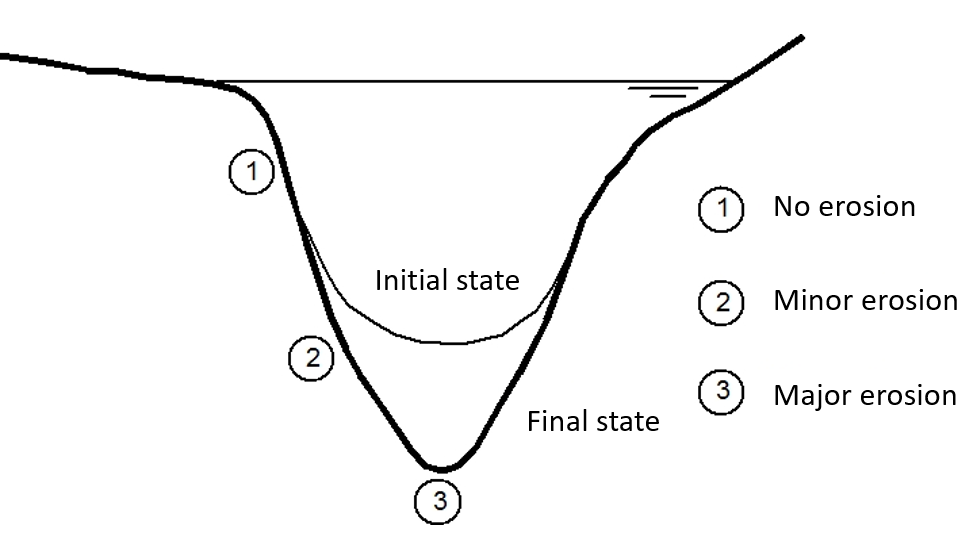
\includegraphics[width=0.7\textwidth]{./graphics/chenal.png}
	\caption{Channel erosion with \courlis without slope stability model}
	\label{fig:no_stab_model}
\end{figure}

This model, based on a single threshold, remains simple and can still be improved. 

\begin{WarningBlock}{Warning}
	The user should also be aware that initial states can be unstable (initial geometry slopes higher than the stability slope) and therefore generate high, non-physical, sediment transport rates at the beginning of the simulation (mainly with \Csuspension). 
\end{WarningBlock}
%%%%%%%%%%%%%%%%%%%%%%% Coupling %%%%%%%%%%%%%%%%%%%%%%%
\subsection{Coupling between \courlis and \mascaret}
\label{coupling}
\begin{figure}[hbt!]
	\centering
	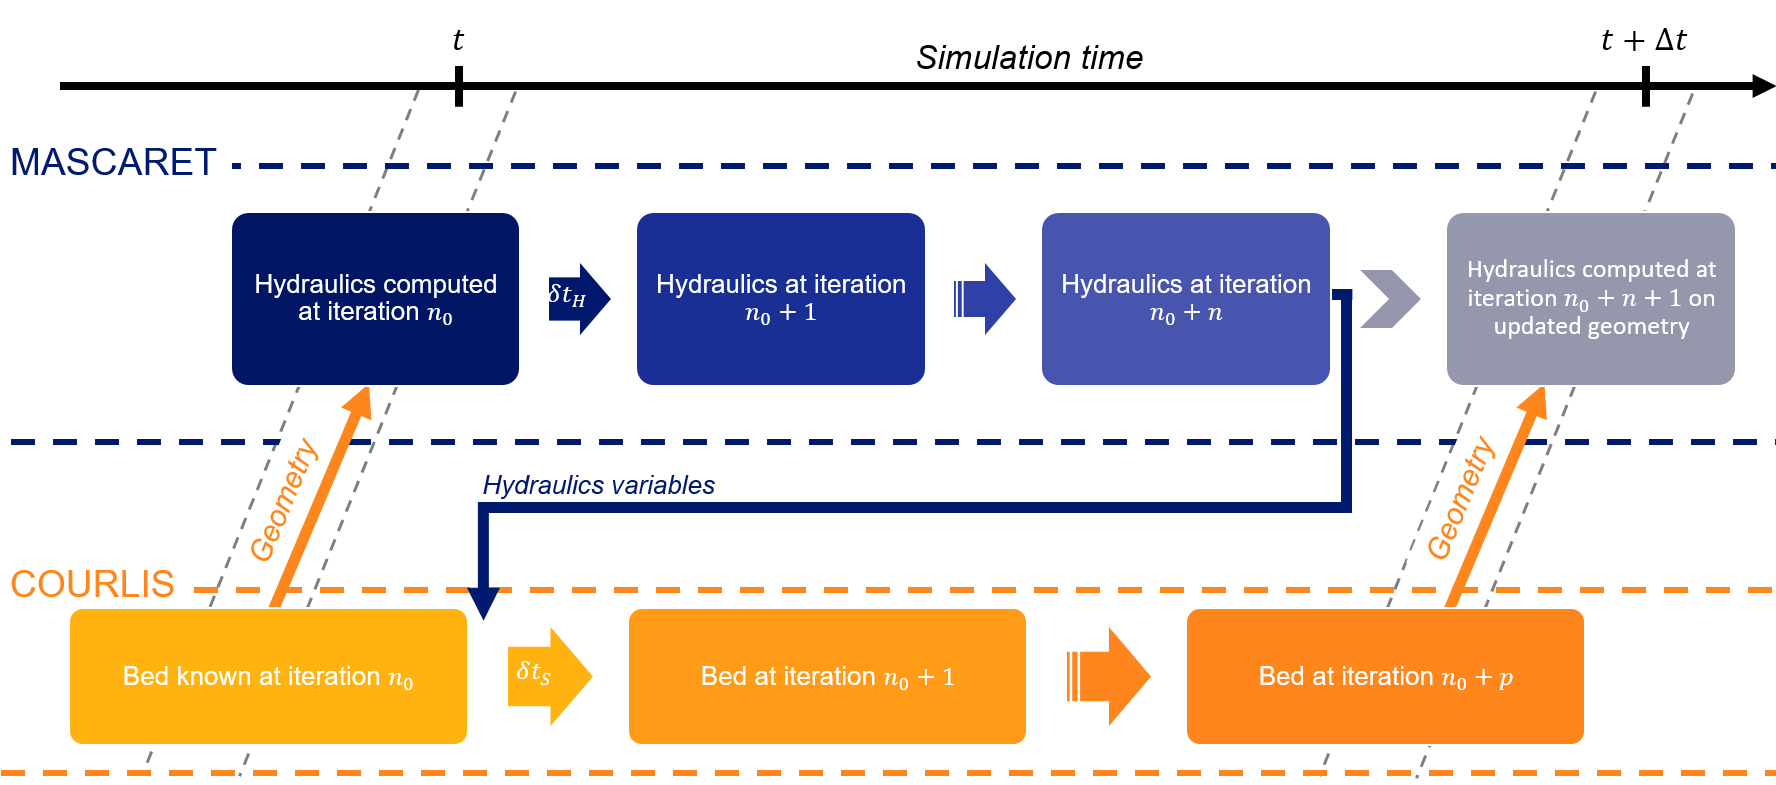
\includegraphics[width=\textwidth]{./graphics/coupling.png}
	\caption{Coupling between \courlis and \mascaret over a time $\Delta t = p \delta t_S = n \delta t_H$}
	\label{fig:coupling}
\end{figure}

The coupling between \courlis and \mascaret is weak. 
Shallow water equations are solved independently by the \mascaret kernel during $n$ timesteps. Hydraulics variables are used by \courlis for solid transport calculations and bed evolutions are given back to \mascaret after $p$ timesteps. Each code uses its own timestep $\delta t_H$ and $\delta t_S$. The hydraulics timestep $\delta t_H$ is chosen by the user while the solid transport timestep $\delta t_S$ is set such as :
$\Delta t = p \delta t_S = n \delta t_H$
The coupling parameters $p$ and $n$ are chosen by the user according to bed evolutions magnitude and speed. 

When the transcritical kernel of \mascaret (also called MASCARET) is used, the hydraulics timestep $\delta t_H$ can vary to match a Courant-Friedrich-Levy number set by the user (traditionally $CFL = 0.8$). 
This Courant-Friedrich-Levy number can reduce computational time as it adapts the hydraulics timestep to spacestep and hydraulics variables values at each iteration:
\bequ
	CFL = \left(  U+\sqrt{gH} \right)  \frac{\delta t_H}{\delta x}
	\label{eq:CFL}
\eequ
In this case, the sediment transport timestep $\delta t_S$ also varies during simulation accordingly. 

\nomenclature{$\delta t_H$}{Hydraulics timestep \nomunit{$s$}}
\nomenclature{$\delta t_S$}{Sediment transport timestep \nomunit{$s$}}




\newpage
%----------------------------------------------------------------------------------------
%	CHAPTER 1b: Evolution of the river cross-section
%----------------------------------------------------------------------------------------
\chapter{Evolution of cross-section}\label{chap1b}
\section{Introduction}

As we can see before, the sediment mass conservation equation, i.e. Exner equation \eqref{eq:exner}, only describes the time-evolution of $Z_b$ which is the bottom elevation (the lowest point of the river cross-section). More precisely, the numerical scheme \eqref{eq:exner-scheme} computes
\begin{equation}\label{eq:exner-sediment-volume}
\Delta V_i^{n+1} \equiv V_i^{n+1} - V_i^n
\end{equation}
the eroded/deposited volume of sediments at cell $i$ during the time $t^n$ to time $t^{n+1}$. As a consequent, an additional closure is needed in order to describe the evolution of river cross-section.

Several closures can be found in the literature. The simplest closure may be a {\em flat} deposition and an {\em uniform} erosion; the height of erosion at each point on the river cross-section can even be weighted in according with the efficient shear stress $\tau_{eff}$. An another one consists in applying an uniform evolution for both deposition and erosion cases.

Once the geometry of cross-sections are modified by erosion or deposition, the {\em planimetrage functions} -- vertical discretization of cross-sections -- need to be re-calculated at each time step
\begin{itemize}
\item $B(z)$: width of cross-section,
\item $S(z)$: area of cross-section,
\item $P(z)$: perimeter of cross-section,
\end{itemize}
corresponding to a given elevation $z$. As remarked before, this becomes costly for long-term simulations with a lot of bed evolutions (which can represent up to more than 90\% of the total calculation time of \courlis).

In the following, we are interested by the simple closures allowing direct analytic computation of planimetrage functions $B^{n+1}, S^{n+1}, P^{n+1}$ at time $t^{n+1}$ from time $t^n$ (available  functions $B^n, S^n, P^n$), or from the initial time $t^0$ (functions $B^0, S^0, P^0$ are given by \mascaret after initialization step).  The choice of these closures is given with the keyword \telkey{OPTION D'EVOLUTION DE PROFIL} or \telkey{OPTION FOR PROFILE EVOLUTION}.

\section{Option 1: uniform erosion -- flat deposition}

\subsection{Keywords}
\begin{itemize}
\item \telkey{OPTION FOR PROFILE EVOLUTION = 1} (default)
\end{itemize}

\subsection{Profile evolution}
Evolution of the river bottom is not applied in the same way for erosion and for deposition :
\begin{itemize}
 \item Evolution due to erosion is applied uniformely on all points of the river bottom located under the free surface ;
 \item Evolution due to deposition is applied horizontally (at constant elevation). For each horizontal deposition surface, the corresponding elevation is computed by linear interpolation of the curves generated by vertical discretization (cf Section \ref{planim}).
\end{itemize}

\begin{figure}[htb!]
    \centering
    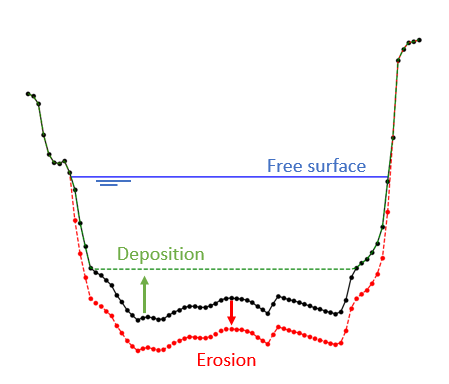
\includegraphics[width=0.45\textwidth]{./graphics/erosion_deposition.png}
    \caption{Flat deposition and uniform erosion}
    \label{fig:depo_ero2}
\end{figure}

\subsection{Planimetrage functions}
wip

\section{Option 2: uniform erosion -- uniform deposition}

\subsection{Keywords}
\begin{itemize}
\item \telkey{OPTION FOR PROFILE EVOLUTION} = 2
\item \telkey{FILE FOR THE WIDTH OF EROSION} = largeur.xlim
\end{itemize}

\subsection{Profile evolution}
For a cross-section $i$, a value $B_i$ {\em width of erosion} or the positions $x_i^L, x_i^R$ on the left and the right river banks have to be prescribed in the \telkey{FILE FOR THE WIDTH OF EROSION}. The format of this later file is closely derived from that of geoCourlis as follows:

\begin{figure}[htb!]
\begin{verbatim}
Profil Bief_1 Profil_1 X1     Profil Bief_1 Profil_1 X1 [B1 or X1L X1R]
Profil Bief_1 Profil_2 X2     Profil Bief_1 Profil_2 X2 [B2 or X2L X2R]
...                           ...
\end{verbatim}
\caption{geoCourlis file (left) and (right) format of \telkey{FILE FOR THE WIDTH OF EROSION}.}
\end{figure}

The mechanism for erosion and deposition cases are illustrated on Fig. \ref{fig:option-uni-depo-ero}. The current geometry is derived from initial cross-section. In the case of erosion, the part of initial cross-section lying between $x^L$ and $x^R$ is uniformly displaced downward with a thickness $\delta z_i$. For the opposed case, this part of initial cross-section is uniformly moved upward by $\delta z_i$ and completed by horizontal jonctions at $x^L$ and $x^R$.

\begin{figure}[htb!]
    \centering
    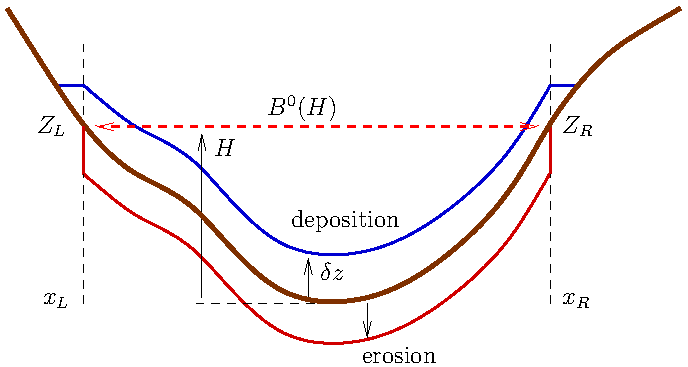
\includegraphics[width=0.5\textwidth]{./graphics/option-uni-depot-ero.pdf}
    \caption{Uniform deposition and uniform erosion, with the brown curve corresponding to the initial profile}
    \label{fig:option-uni-depo-ero}
\end{figure}

\subsection{Planimetrage functions}
The planimetrage functions $B^{n+1}, S^{n+1}, P^{n+1}$ can be directly computed from those of initial time $B^0, S^0, P^0$.

First, we compute from $B^0$ the height $H_i$ associated to the given width of erosion $B_i$ by solving
\begin{equation}\label{eq:height-of-erosion}
  B_i=B_i^0(H_i).
\end{equation}

Given a volume of sediment $\Delta V_i^{n+1}$ (by \eqref{eq:exner-sediment-volume}), we next compute $\delta z_i$ the thickness of evolution and $B^{n+1}, S^{n+1}, P^{n+1}$ resulting from the conservation of sediment the cross-section:
\begin{itemize}
\item Erosion $(V_i^{n+1} \leq 0)$
  \begin{equation}\label{eq:thickness-of-erosion}
\Delta V_i^{n+1} = B_i\delta z_i\Delta x,
  \end{equation}
For a height $z$ from the bottom elevation $Z_b$,
  \begin{align*}
    	& S_i^{n+1}(z) = \left\{\begin{array}{lll}
	S_i^0(z) & \text{if} & z \leq H_i, \\
	S_i^0(H_i) + (z-H_i)B_i & \text{if} & H_i \leq z \leq H_i + \delta z, \\
	S_i^0(z-\delta z_i) + B_i\delta z_i & \text{else.}
	\end{array}\right. \\
	& B_i^{n+1}(z) = \left\{\begin{array}{lll}
	B_i^0(z) \hspace*{2cm} & \text{if} & z \leq H_i, \\
	B_i^0(H_i) & \text{if} & H_i \leq z \leq H_i + \delta z, \\
	B_i^0(z-\delta z_i) & \text{else.}
	\end{array}\right.\\
	& P_i^{n+1}(z) = \left\{\begin{array}{lll}
	P_i^0(z) & \text{if} & z \leq H_i, \\
	P_i^0(H_i) + 2(z-H_i) & \text{if} & H_i \leq z \leq H_i + \delta z_i, \\
	P_i^0(z-\delta z_i) + 2\delta z_i & \text{else.}
	\end{array}\right.
  \end{align*}

\item Deposition $(V_i^{n+1} > 0)$
   \begin{equation}\label{eq:thickness-of-deposition}
\Delta V_i^{n+1} = S_i^0(H_i + \delta z_i) - S_i^0(H).
   \end{equation}
For a height $z > 0$ from the bottom elevation $Z_b$,
   \begin{align*}
	& S_i^{n+1}(z) = \left\{\begin{array}{lll}
	S_i^0(z) & \text{if} & z \leq H_i, \\
	S_i^0(z+\delta z_i) - \Delta V_i^{n+1} & \text{else.}
	\end{array}\right. \\
	& B_i^{n+1}(z) = \left\{\begin{array}{lll}
	B_i^0(z) \hspace*{2cm} & \text{if} & z \leq H_i, \\
	B_i^0(z+\delta z_i) & \text{else.}
	\end{array}\right. \\
	& P_i^{n+1}(z) = \left\{\begin{array}{l}
	P_i^0(z) \hspace*{2cm} \text{if} \quad z \leq H_i, \\
	P_i^0(z+\delta z_i) + \Big[B_i^0(H_i+\delta z_i) - B_i\Big] - \Big[P_i^0(H_i+\delta z_i) - P_i^0(H_i)\Big].
	\end{array}\right.
	\end{align*}
\end{itemize}

\newpage
%----------------------------------------------------------------------------------------
%	CHAPTER 2: Pre-treatment
%----------------------------------------------------------------------------------------
\chapter{Pre-treatment}\label{chap2}
\section{PreCourlis}
wip

\section{Pretel}
wip

\newpage

%----------------------------------------------------------------------------------------
%	CHAPTER 3: The inputs
%----------------------------------------------------------------------------------------
\chapter{The inputs}\label{chap3}
To run a simulation, at least 4 files are needed :
\begin{itemize}
	\item The \cas for \courlis [Section \ref{cas_files}]
	\item The \xcas for \mascaret [Section \ref{cas_files}]
	\item The geometry file for \mascaret (\telfile{geometry.geo}) [Section \ref{geo_file}]
	\item The sediment layers file for \courlis (\telfile{geometry.geoC}) [Section \ref{geoC_file}]
\end{itemize}
Additional inputs can be used to specify liquid and solid boundary conditions or initial states. 

\section{The cas and xcas files}
\label{cas_files}
\subsection{Current set-up}
The \xcas containing \mascaret set up information can be adapted from \mascaret calculations or generated thanks to \fudaa (available at \url{www.opentelemac.org}). The reader can refer to the \mascaret guide for more information.

From a \mascaret file, the \courlis module is activated by modifying xml lines in the \xcas as described below :

\begin{figure}[htb!]
    \centering
    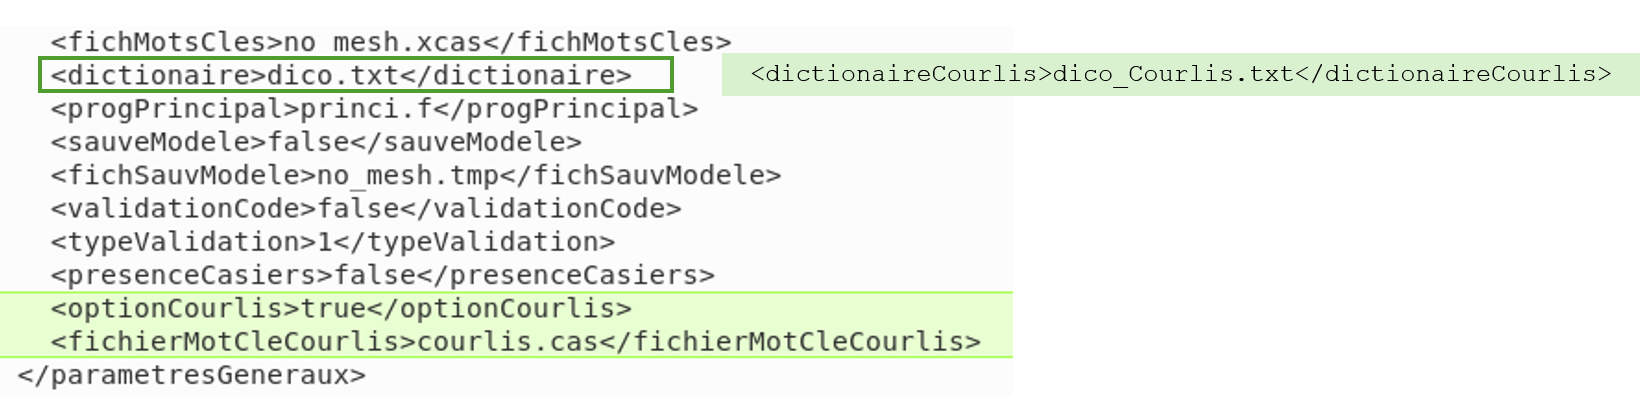
\includegraphics[width=0.9\textwidth]{./graphics/xcas_courlis.png}
    \caption{Changes in the \xcas to activate \courlis}
    \label{fig:xcas}
\end{figure}

First, the \courlis dictionary replaces the \mascaret one. Two lines are added to specify the activation of \courlis (\telkey{<optionCourlis>true</optionCourlis>}) and the name of the \courlis \cas (in this example called \telfile{courlis.cas}). 
These changes will call the \courlis routines with the parameters given in the corresponding \cas. \courlis can be shut off at any time by setting \telkey{<optionCourlis>false</optionCourlis>} resulting in a traditionnal \mascaret simulation. 

An example of an \xcas is given in Appendix \ref{app:xcas}. 

\begin{WarningBlock}{Warning}
	\fudaa provides an interface to generate \xcass but since \fudaa v7p2, the software is no longer supported. Consequently, 4 tags xml are missing from \xcass generated with \fudaa :
	\begin{itemize}
		\item	The \courlis dictionnary tag (Figure \ref{fig:xcas})
		\item 	The \courlis option tag (Figure \ref{fig:xcas})
		\item	The \courlis key file tag (Figure \ref{fig:xcas})
		\item 	The uncentered scheme option tag for the permanent kernel of \mascaret (Figure \ref{fig:xcas_decentrement})
	\end{itemize}
	If a \fortran error (\verb"At line 531 of file .../pretrait.f90") appears while running \mascaret with SARAP it may be that the recently developed option of uncentered scheme for this kernel has not been added to the \xcas.
\end{WarningBlock}

\begin{figure}[htb!]
    \centering
    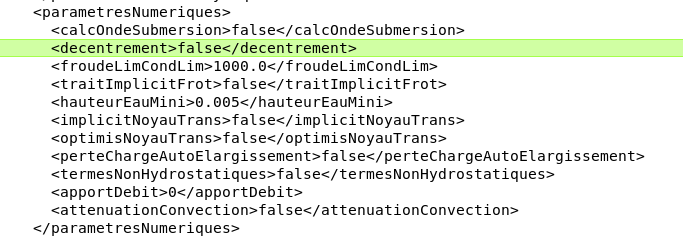
\includegraphics[width=0.8\textwidth]{./graphics/decentrement_xcas.png}
    \caption{Changes in the \xcas to add the uncentered option (set to \telkey{TRUE} to activate it)}
    \label{fig:xcas_decentrement}
\end{figure}

The \cas put in the \xcas controls \courlis parameters.
\courlis keywords, gathered in this file, are presented in the next sections.
An example is given in Appendix \ref{app:cas}. 

\subsection{Coming set-up}
Soon the code will only parse \xcass, one for \mascaret and one for \courlis, and no longer one \xcas for \mascaret and one \cas for \courlis. Nevertheless, thanks to \python script, the user will have the choice to launch the calculation with two \cass or two \xcass.

This improvement will make \mascaret parameters more readable and intuitive to facilitate its use.
\xcass can be converted to \cas via the command \\
\verb|manip_cas.py xcas2cas_1d <my_xcas_file.xcas> <output_cas_file.cas>|.

\begin{CommentBlock}{Warning}
	The keywords are not yet all translated in the dictionnary. So, in v8p3, this conversion will make a mixed english/french \cas !
\end{CommentBlock}

%%%%%%%%%%%%%%%%%%% GEOMETRY %%%%%%%%%%%%%%%%%%%%%
\section{Geometry and sediment layers}
\label{sedi_layers}

\subsection{The .geo file}
\label{geo_file}

The geometry file contains the initial bottom elevations of the reach, i.e. the initial elevation of the interface between the bottom and the water. 
Simple geometries can be generated thanks to \fudaa. Extraction of profiles from bathymetric measurements can be done thanks to \precourlis\footnote{In QGIS : \url{https://plugins.qgis.org/plugins/PreCourlis/} or GitHub : \url{https://github.com/msecher/PreCourlis}}.
While using \courlis, no mesh can be generated during simulation. That is why, unlike \mascaret, the cross-sections must be interpolated in pre-treatment.
If the space step of the geometry is not sufficient, interpolation can also be done with \precourlis.

\begin{CommentBlock}{Warning}
	It is recommended to avoid as much as possible vertical walls in geometry when using \courlis. Indeed, some approximations are done by \mascaret when lateral walls are vertical and hydraulics errors will be amplified by \courlis calculations. 
\end{CommentBlock}

\subsection{The .geoC file}
\label{geoC_file}

The \courlis geometry file contains the initial elevations of the different sediment interfaces. 

For each cross-section, the first column corresponds to the bottom layer as specified in the \telfile{geo file}. The next columns correspond to the different interfaces between sediment layers (as shown below). The last column corresponds to a non-erodable substratum (hard bottom). 
With the suspension module, two virtual layers are commonly set to represent sand and silt transport i.e. the initial width of these two layers is null. A third layer can be added to represent sediment already present in the initial step. This configuration corresponds to 4 interfaces in the \telfile{geoC file} as represented below
When modeling bedload, only one layer is useful and therefore 2 interfaces are given in the \telfile{geoC file} as represented below. 

\begin{figure}[htb!]
    \centering
    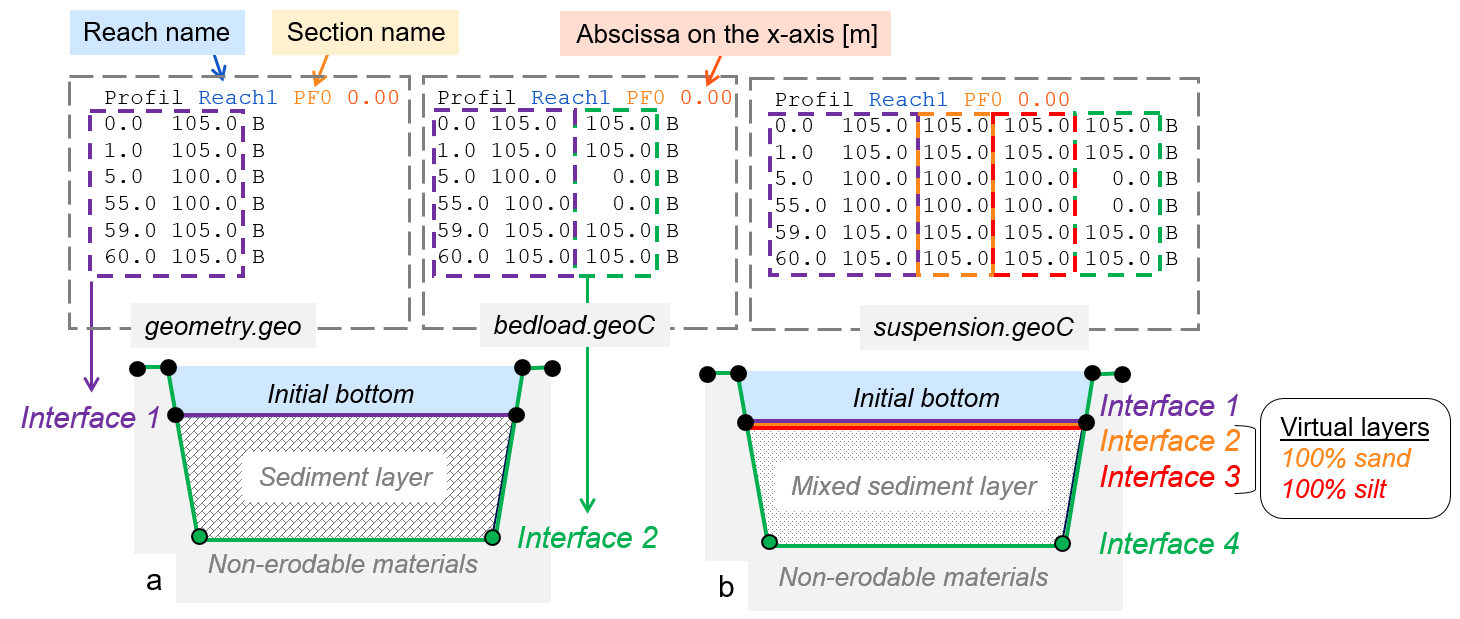
\includegraphics[width=\textwidth]{./graphics/geo_files.png}
    \caption{Examples of one cross-section in the \telfile{geo and geoC files} for (a) bedload and (b) suspension simulations}
    \label{fig:geo_files}
\end{figure}

\section{Optional inputs}
\label{optional_inputs}

Hydraulics boundary conditions are often written in an external file, for example \telfile{hydrograph.loi} at the upstream boundary and \telfile{elevation.loi} at the downstream boundary. Initial free surface elevations can also be given in an external file for example called \telfile{init.lig}. All external files names are specified in the \xcas. The reader can refer to the \mascaret guide for more information.\\

Similarly, sediment concentrations at boundaries can be given to \courlis from external files, for example \telfile{qs.loi}. The corresponding \telkey{LOI CONC X MODE D''ENTREE} keyword, with \telkey{X} the law number, should be set to \telkey{1} in the \cas (and conversely to \telkey{2} if the information is given directly in the \cas). The name of the files are then given by \telkey{LOI CONC X FICHIER}.\\

Initial concentrations for \Csuspension can be set into an external file : 
\begin{itemize}
	\item \telkey{MODE D'ENTREE DES CONCENTRATIONS INITIALES POUR COURLIS = 1} (by default)
	\item \telkey{FICHIER DES CONCENTRATIONS INITIALES POUR COURLIS} : the external file name
\end{itemize}

In addition, sediment characteristics can also be given in an external file :
\begin{itemize}
	\item \telkey{MODE D''ENTREE DES CARACTERISTIQUES SEDIMENTAIRES = 1} (by default)
	\item \telkey{FICHIER DES CARACTERISTIQUES SEDIMENTAIRES} : the external file name
\end{itemize}

\begin{WarningBlock}{French-English keywords}
	Keywords were first developed in French. Translation of keywords in English has been started (\telfile{sources/mascaret/mascaret.dico}) but is not yet available in the code. Consequently, the following sections will present the French keywords and the corresponding English keywords when they are available in \courlis v8p3 (listed in the \verb|dico_Courlis.txt| generated when launching a \courlis simulation).
\end{WarningBlock}


\newpage

%----------------------------------------------------------------------------------------
%	CHAPTER 4: General Setup
%----------------------------------------------------------------------------------------
\chapter{General setup}\label{chap4}
\chapter{General setup of the hydrodynamic computation (Navier-Stokes equations)}

The general setup of the computation is only performed at the steering file
level.

The time data is provided by the two keywords \telkey{TIME STEP} (real, set at
1. by default) and \telkey{NUMBER OF TIME STEPS}. The first keyword sets the
period of time between two consecutive computational moments (but not
necessarily two outputs in the result file). The global duration of the
computation is provided through a number of time steps (keyword \telkey{NUMBER
OF TIME STEPS}, set at 1 by default) or a duration in seconds (keyword
\telkey{DURATION}, set at 0. by default). If both are given, \telemac{3D} follows
the instruction leading to the longest computation.

By default the initial time is equal to 0.~s.
Since release v8p5, it can be changed by setting the keyword
\telkey{INITIAL TIME} (default = 0.~s).
It avoids to change previous hard-coded value 0. in \telfile{CONDIM} subroutine.
If input data is defined from a specific time and the user wants to start the
computation from another time, it is a way to do it without changing input data.

Both date and hour corresponding to the initial time of the computations can be
specified using the keywords \telkey{ORIGINAL DATE OF TIME}
(AAAA, MM, JJ format; default value = 1900; 1; 1) and \telkey{ORIGINAL
HOUR OF TIME} (HH, MM, SS format, default value = 0; 0; 0).
These two data are mandatory if using the tidal data bases.
They can be taken into account in programming by means of the \telfile{MARDAT}
and \telfile{MARTIM} variables.

The computation title is specified by the keyword \telkey{TITLE}.


\section{Mesh definition}

The three-dimensional mesh, consisting of prisms possibly cut into
%(\telkey{ELEMENT} = 'TETRAHEDRON'
%in that case but the default element for discretization is a prism
%with \telkey{ELEMENT} = 'PRISM'),
tetrahedrons, is automatically constructed by \telemac{3D} from the
two-dimensional mesh. This construction is done in the \telfile{CALCOT}
subroutine from the information given by the subroutine defining the
mesh transformation \telfile{USER\_MESH\_TRANSF} or, by default if using a
classical sigma transformation, in the \telfile{CONDIM} subroutine.

The number of prisms is specified in the steering file by means of the keyword
\telkey{NUMBER OF HORIZONTAL LEVELS} (default value = 2). That number of levels
is equivalent to the number of stacked prisms plus 1. Its minimum value is 2 (1
prism in the vertical direction).

\telemac{3D} uses a change of variables in order to freeze the mesh on a time
step (without such a change, the mesh dimensions $z$ would vary in
accordance with the free surface evolution). The frequently adopted change of
variables is the sigma transform which consists in shifting from the $z(x,y,t)$
co-ordinate to the $z^{*} (x,y)$ co-ordinate.
The user should enter the $z^{*}$ co-ordinates in the \telfile{USER\_MESH\_TRANSF}
subroutine.
The normalized co-ordinates will then range from 0 (the bottom) to 1 (the surface).

The numbering of levels is made according to upward vertical. Level 1 follows
the bottom and level $N$ corresponds to the free surface ($N$
being specified by the keyword \telkey{NUMBER OF HORIZONTAL LEVELS}).

The vertical mesh definition is based on the \telfile{TRANSF\_PLANE} table which
allows defining the behaviour of each level.

The keyword \telkey{MESH TRANSFORMATION} sets the kind of level distribution
along the vertical. The value 0 corresponds to a distribution directly defined
by the user in the \telfile{CALCOT} subroutine.
The default value 1 corresponds to the classical sigma transformation.

\begin{figure}[H]%
\begin{center}
%
  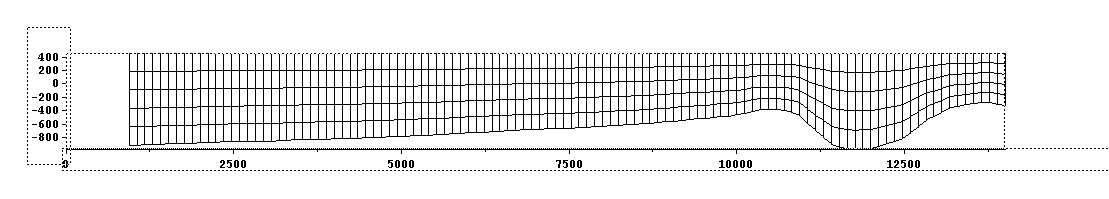
\includegraphics[width=\textwidth]{./graphics/mesh_transformation}
%
\end{center}
\caption
[Effect of the \telkey{MESH TRANSFORMATION}]
{Effect of the \telkey{MESH TRANSFORMATION} keyword -- Value 1: sigma.}
\label{fig:mesh_transf}
\end{figure}

The default value is 1 (Figure \ref{fig:mesh_transf}) and results in a
homogeneous distribution of levels in the vertical direction (classical sigma
transformation). The height of the levels varies depending on the water depth,
all planes can move (except for the bottom). In this case, no programming in
the \telfile{USER\_MESH\_TRANSF} subroutine is required.

A value of 2 (Figure \ref{fig:mesh_transf2}) will allow the user to define the
distribution of levels (e.g. refinement near surface) while maintaining the
levels mobility (sigma transformation with given proportions). The latter
choice implies that the user will program his/her distribution in the
\telfile{USER\_MESH\_TRANSF} subroutine to define the \telfile{ZSTAR} array
that describes
the distribution of levels along the vertical as a percentage of the water depth.
Changes to make are:

\begin{itemize}
\item Specifying the variable \telfile{TRANSF\_PLANE} with a value of 2
for every level,

\item Specifying the level distribution along the vertical through the array
\telfile{ZSTAR} which describes the distribution along the vertical as a
percentage of the water depth (the values are between 0. and 1.).
\end{itemize}

For example (Figure \ref{fig:mesh_transf2}):

\begin{lstlisting}[language=TelFortran]
DO IPLAN = 1,NPLAN
  TRANSF_PLANE%I(IPLAN)=2
ENDDO

ZSTAR%R(1)=0.D0
ZSTAR%R(2)=0.02D0
ZSTAR%R(3)=0.1D0
ZSTAR%R(4)=0.4D0
ZSTAR%R(5)=0.8D0

\end{lstlisting}

\begin{figure}[H]%
\begin{center}
%
  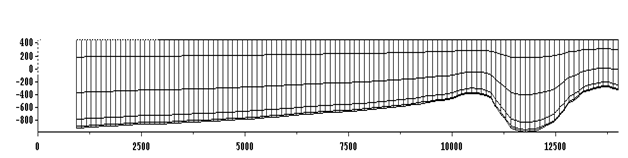
\includegraphics[width=\textwidth]{./graphics/mesh_transformation2}
%
\end{center}
\caption
[Effect of the \telkey{MESH TRANSFORMATION2}]
{Effect of the \telkey{MESH TRANSFORMATION} keyword -- Value 2: zstar.}
\label{fig:mesh_transf2}
\end{figure}

In order to better represent the densimetric stratification areas
(thermoclines, halocline and/or outfall), prescribing a maximum number of
horizontal "levels" (particularly those where the gradients are the highest) is
sometimes suitable. For that purpose, the user can select the value 3 for the
keyword \telkey{MESH TRANSFORMATION}. In this configuration, the user can
freely use the 3 types of level definition available in \telemac{3D} to create
the mesh along the vertical:

\begin{itemize}
\item Fixed levels at a given altitude (correspond to value 3 of the
\telfile{TRANSF\_PLANE} variable, the altitude is specified by the
\telfile{ZPLANE} variable),

\item Irregularly distributed movable levels between two fixed levels
(correspond to value 2 of the \telfile{TRANSF\_PLANE} variable,
the distribution is specified by the \telfile{ZSTAR} variable),

\item Evenly distributed movable levels between two fixed levels (correspond
to value 1 of the \telfile{TRANSF\_PLANE} variable).
\end{itemize}

This latter choice requires the user to make changes in the
\telfile{USER\_MESH\_TRANSF} subroutine:

\begin{itemize}
\item Specifying the variable \telfile{TRANSF\_PLANE} at value 1, 2 or 3
for each level,

\item Specifying the level distribution along the vertical through the array
\telfile{ZSTAR} for levels of type 2,

\item Specifying the level altitude through the array \telfile{ZPLANE}
for levels of type 3.
\end{itemize}

For example (Figure \ref{fig:mesh_transf3}):
\begin{lstlisting}[language=TelFortran]
DO IPLAN = 1,5
  TRANSF_PLANE%I(IPLAN)=2
ENDDO
ZSTAR%R(1)=0.D0
ZSTAR%R(2)=0.2D0
ZSTAR%R(3)=0.5D0
ZSTAR%R(4)=0.7D0
ZSTAR%R(5)=0.8D0

DO IPLAN = 7,NPLAN
 TRANSF_PLANE%I(IPLAN)=1
ENDDO

TRANSF_PLANE%I(6)=3
ZPLANE%R(6)=0.D0
\end{lstlisting}

\begin{figure}[H]%
\begin{center}
%
  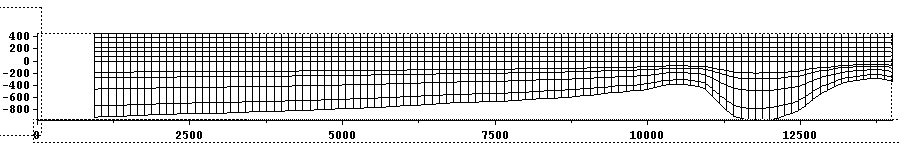
\includegraphics[width=\textwidth]{./graphics/mesh_transformation3}
%
\end{center}
\caption
[Effect of the \telkey{MESH TRANSFORMATION3}]
{Effect of the \telkey{MESH TRANSFORMATION} keyword -- Value 3: user defined.}
\label{fig:mesh_transf3}
\end{figure}

Various programming examples are provided as comments in the
\telfile{USER\_MESH\_TRANSF} subroutine.\\

The triangular based prismatic elements can optionally be split into
tetrahedrons. This option is enabled using the \telkey{ELEMENT} keyword can
take the value 'PRISM' (default value) or 'TETRAHEDRON'.\\

There are some divisions by 3D volumes in the \telfile{MESH\_PROP} subroutine.
A minimum volume value can be set with the keyword
\telkey{MINIMUM VOLUME OF 3D ELEMENTS} expressed in m$^3$
(default = $10^{\rm{-6}}$~m$^3$ = 1~cm$^3$).
This value can be changed, for example when modelling scale experiments where
dimensions are not big (total length of the order 1~m or less).\\

When using \telkey{MESH TRANSFORMATION} = 3, for all or several planes,
the distance between this kind of planes are spaced with a minimum value.
Close to the bottom, this minimum distance between planes can be set with the
keyword \telkey{MINIMUM DISTANCE BETWEEN PLANES CLOSE TO THE BOTTOM}
whereas close to the free surface, this minimum distance can be set with the
keyword \telkey{MINIMUM DISTANCE BETWEEN PLANES CLOSE TO THE FREE SURFACE}.
By default, each distance is set to 0.2~m.

The keyword \telkey{THRESHOLD HEIGHT BEFORE CRUSHED ELEMENTS} can be used
to decide below which height the 3D elements are treated as crushed.
This is not done for the free surface plane.
The default value 0~m means there are no elements treated as crushed
(outside tidal flats).
With constant elevation planes, to have crushed elements at the bottom rather
than elements at the bottom with a minimum height of
\telkey{MINIMUM DISTANCE BETWEEN PLANES CLOSE TO THE BOTTOM},
this last keyword should be set to 0~m and
\telkey{THRESHOLD HEIGHT BEFORE CRUSHED ELEMENTS} to a value greater than 0~m.
\\

Another mesh transformation was introduced in release 6.1:
the Adaptive Mesh Refinement (or Redistribution) aka AMR.
It can be used by setting \telkey{MESH TRANSFORMATION} = 5.
The mesh is changed following criteria for a tracer.
The interested user can read the TUC 2011 proceeding \cite{Cawthorn2011}
for more details.
The keyword \telkey{NUMBER OF TRACER FOR AMR} enables to change the number of
tracer given to AMR algorithm in order to adapt the vertical mesh (default = 1).


\section{Prescribing the initial conditions}

The initial conditions aim at defining the model condition at the beginning of
the simulation.

In case of a continuing computation, the initial conditions are provided at one
time step in the result file of the previous computation (refer to section
\ref{sec:previousfile}).
The mandatory variables (at least the velocity components) when resuming
the computation should then have been stored into the file being used as
\telkey{PREVIOUS COMPUTATION FILE}.

Otherwise, the default initial condition is defined as follows:

\begin{itemize}
\item Free surface set to an elevation equal to 0,

\item Zero velocities,

\item Steady zero active and passive tracers.
\end{itemize}

If that initial condition is not suitable for a computation, then it should be
changed using keywords in the simple cases or through a programming as
described in the subsequent subsections.


\subsection{Prescription through keywords}

In all the cases, the kind of initial conditions is set by the keyword
\telkey{INITIAL CONDITIONS}. That keyword can have one of the following six
values:

\begin{itemize}
\item 'ZERO ELEVATION': Initializes the free surface elevation
to 0 (default value). The initial water depths are then computed from the
bottom elevation,

\item 'CONSTANT ELEVATION': Initializes the free surface elevation to the
values as supplied by the keyword \telkey{INITIAL ELEVATION}
(default value = 0.). The initial water
depths are then computed by getting the difference between the free surface
elevation and the bottom elevation.
In those areas where the bottom elevation exceeds
the initial elevation, the initial water depth is zero,

\item 'ZERO DEPTH': All the water depths are initialized with a zero value
(free surface coinciding with bottom). In other words, the whole domain is
"dry" at the beginning of the computation,

\item 'CONSTANT DEPTH': Initializes the water depths to the value as supplied
by the keyword \telkey{INITIAL DEPTH} (default value = 0.),

\item `TPXO SATELLITE ALTIMETRY': The initial conditions are set using
information provided by the OSU harmonic constants database (TPXO for instance)
or HAMTIDE model
in the case of the use of this database for the imposition of maritime boundary
conditions (see subsection \ref{sec:tide}),

\item 'PARTICULAR' or 'SPECIAL': The initial conditions for water depth/
free surface are defined as programmed by the user
in the \telfile{USER\_CONDI3D\_H} subroutine (refer to the next
subsection).
That procedure should be used whenever the initial conditions of the model do
not correspond to one of above five cases.
\end{itemize}


\subsection{Prescribing particular initial conditions with user subroutines}
% (Programming the \telfile{USER\_CONDIM\_}... subroutines)
\label{sec:prescr_IC}

The \telfile{USER\_CONDI3D\_H}, \telfile{USER\_CONDI3D\_UVW},
\telfile{USER\_CONDI3D\_TRAC}\ldots
subroutines should be programmed whenever the initial
conditions programmed by default are to be modified.

By default, the standard version of the \telfile{USER\_CONDI3D\_H} subroutine
stops the computation if the keyword \telkey{INITIAL CONDITIONS} is set to
'PARTICULAR' or 'SPECIAL' without any actual amendment of the subroutine.

The \telfile{CONDIM} subroutine successively initializes the two-dimensional
variables, then the three-dimensional variables:

\begin{itemize}
\item The water depth,

\item The 3D component of velocities,

\item The active and passive tracers.
\end{itemize}

The user can quite freely fill that subroutine. For instance, he/she can
retrieve information in a formatted or binary file, using the corresponding
keywords.


\subsection{Resuming the computation}

\telemac{3D} enables the user to resume a computation by taking as the initial
condition one time step of a computation which was previously computed on
the same mesh, or possibly with a different number of levels. Thus, some
computational parameters such as the time step, some boundary conditions, the
turbulence model can be modified, or else a computation can be initiated once a
steady state is achieved.

The file to be retrieved shall then inevitably contain all the data required
for \telemac{3D}, i.e. not only the co-ordinates of the $X$, $Y$
and $Z$ computational points which it necessarily contains, but also the
3D velocities and the tracers.

If some variables do not appear in the \telkey{PREVIOUS COMPUTATION
FILE}, then they are automatically set to zero values.  A usual application
consists in using the result of a hydrodynamic computation in order to perform
a tracer transport computation. Generally, the \telkey{PREVIOUS COMPUTATION
FILE} does not include any result for the tracer.

To resume a computation, it is required to use two keywords into the steering
file.

The keyword \telkey{COMPUTATION CONTINUED} should be set to the YES value
(default value = NO).

The keyword \telkey{PREVIOUS COMPUTATION FILE} should provide the name of the
file which will provide the initial conditions.

Optionally, the keyword \telkey{RECORD NUMBER FOR RESTART} can be used to
define the record number to read if it is not the last one (defined by a
default value set to -1).

\begin{WarningBlock}{Warning:}
The two-dimensional mesh on which the useful results have been computed should
be strictly identical to the mesh of the case to be handled.
\end{WarningBlock}

Resuming the computation usually leads to small differences in results
compared to the same calculation without interruption. This difference is
mainly due to the fact that the velocity advection is not treated properly at
the first time step, because this operation requires information from the
previous time step. To correct this, the user has a specific recovery procedure
to improve the accuracy of calculations, using double precision format SERAFIN
files:

\begin{itemize}
\item In the first computation, the keyword \telkey{RESTART MODE} is set to
YES (default = NO),
which generates a specific file containing the full information at one or a
few time step(s) of the simulation (in particular information on the
advection field of the last time step). The name of this file is specified
using the keyword \telkey{RESTART FILE},

\item In the second computation, this specific file must be used as
\telkey{PREVIOUS COMPUTATION FILE} specifying the \telkey{PREVIOUS COMPUTATION
FILE FORMAT} is 'SERAFIND' (SERAFIN double precision).
If the restart should be done from the last time step saved in the
\telkey{RESTART FILE}, the keyword \telkey{RECORD NUMBER FOR RESTART} is to be
let to default value (= -1), otherwise it should be changed.
\end{itemize}

In the first computation, there are 2 keywords which can enable to tune the
resuming of the computation (since release 8.4):
\begin{itemize}
\item If wanting to generate a \telkey{RESTART FILE} at a specific number of
time step different from the last one, the keyword
\telkey{RECORD NUMBER IN RESTART FILE} is to be used
(default = -1 means the \telkey{RESTART FILE} is only written at the last
time step or periodically at the period \telkey{RESTART FILE PRINTOUT PERIOD}),
\item If wanting to generate a \telkey{RESTART FILE} periodically to secure a
file to resume computation in case of crash e.g., the keyword
\telkey{RESTART FILE PRINTOUT PERIOD} defines the printout period in number of
time steps.
Default = 0 means no periodic writing and variables are only written at the last
time step of the computation or at the time step number
\telkey{RECORD NUMBER IN RESTART FILE} if not equal to -1).
\end{itemize}

However, it has to be mentioned that even if it is not advisable, the creation
of specific restart file can be done not only SERAFIND format, but also with
any other available format in the TELEMAC system, especially in single
precision. In this case, the keyword \telkey{RESTART FILE FORMAT} (by default
set at 'SERAFIND') must be set to the proper value.

A particular aspect of the resuming technique of computation is the value of
the start time of the second simulation. By default, the start time of the
second calculation is equal to the value of the last time step of restart file.
This can be changed by using the logical keyword \telkey{INITIAL TIME SET TO
ZERO} if the user wants to start from zero (default value is NO).
\\

It is also possible to resume a computation from a 2D results file. This is
generally useful in river hydraulic offering the possibility to initialise the
model in 2D before shifting to 3D simulation. In this case, the horizontal
velocities are considered as constant on the vertical and equal to the 2D
velocities and the vertical velocities are initialised to zero. This
possibility is activated using the \telkey{2D CONTINUATION} logical keyword
(default value = NO). The 2D results file must be given using \telkey{FILE FOR
2D CONTINUATION}. The keyword \telkey{FILE FOR 2D CONTINUATION FORMAT} gives
the format of the file and can takes the following values: `SERAFIN ' (default
value), `SERAFIND' and `MED'.

Since release 8.5, if \telkey{2D CONTINUATION} = YES and the
\telkey{FILE FOR 2D CONTINUATION} contains bottom friction data, these values
are taken into account rather than the potential ones in the
\telkey{GEOMETRY FILE}.

\section{Prescribing the boundary conditions}
\label{sec:prescr_BC}

The boundary conditions are handled through types of conditions which are
related to the computational variables. The combination of these types (from a
list of possible choices) describes whether the boundary is liquid or solid and
how it should be processed.

In \telemac{3D}, the water depth $H$, the horizontal velocities $U$
and $V$ and the tracers are the only variables which necessarily involve
defining their type of boundary conditions. Those types of boundary conditions
applicable to the vertical velocity and the $k$ and $\epsilon$ functions
are managed by \telemac{3D} by the user directly in the FORTRAN source files of
\telemac{3D} and therefore do not have a type. If the computation takes tracers
into account, then a single type (common to all the tracers) should also be
defined for a given boundary.

Once all the types of the boundary are defined, the user should enter the
related values for the computational variables (at least $H$, $U$ and $V$).

For example, the user may want to set the sea level and leave the velocity
field free (e.g. the tide case). The type of boundary will be: "prescribed
depth and free velocity". The values required for that type are only water
depth at every instant at that boundary. The values of velocities (if they are
entered) are not taken into account for that boundary.

Thus, for each \telemac{3D} boundary, the computational variables (at least
$H$, $U$ and $V$) are necessarily associated with one type
and each type may be associated with one value (either used or not).

The maximum number of boundaries is set to 30 by default but it can be changed
by the user with the keyword \telkey{MAXIMUM NUMBER OF BOUNDARIES}.
This avoids changing the previously hardcoded values (until release 7.0),
which required recompiling the whole package.

After such a description of what is a boundary in \telemac{3D}, we will describe
the types, then the related values.

\subsection{The boundaries in \telemac{3D}}

Water depth is the only two-dimensional variable computed. Its processing at
the boundaries is like that being performed by \telemac{2D}. The boundary points
to be handled are those of the two-dimensional mesh (refer to Figure
\ref{fig:bnd}).

For the other variables (velocities and tracers), the boundary conditions
should be handled over all the boundaries of the three-dimensional mesh which
includes:

\begin{itemize}
\item The lateral boundary points (vertical column points linked to the
boundaries of the two-dimensional mesh), whether it is a liquid or solid
boundary,

\item The points belonging either to the free surface or the bottom.
\end{itemize}

\begin{figure}[H]%
\begin{center}
%
  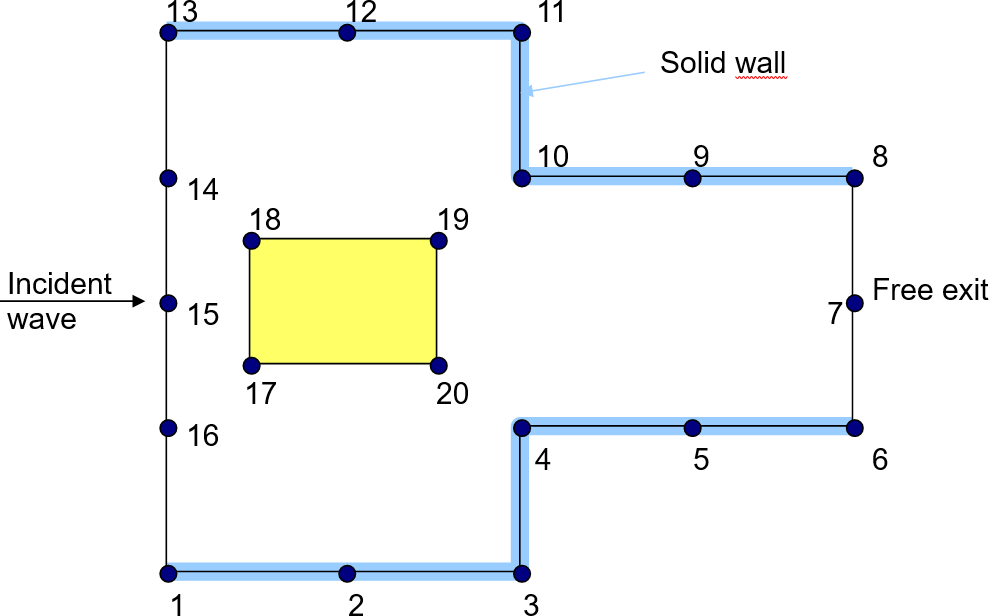
\includegraphics[width=0.7\textwidth]{./graphics/bnd}
%
\end{center}
\caption
[Boudnaries in \telemac{3D}]
{The various boundaries in \telemac{3D} (bridge piers case study).}
\label{fig:bnd}
\end{figure}

By default, \telemac{3D} automatically handles all the surface and bottom points
which do not belong to the side walls. The user, however, can modify them. This
can be done by modifying the FORTRAN sources.

All the remaining points (on the lateral boundaries) are linked to the
two-dimensional mesh boundaries at each horizontal level. Thus, they will be
processed in a similar fashion as in \telemac{2D}. The number of required data,
however, increases so much that a full external handling (either through the
steering file or the boundary conditions file) would become excessively
complex. That is why the range of options offered to the user for dealing with
these boundary conditions is narrower than in \telemac{2D} and definitely implies
programming the sources of the user-available software. The next following
subsections describe the way the boundary nodes are handled.


\subsection{The boundary-related types}

The boundary condition type for $H$, $U$, $V$ and $T$ of the edge points is
read in the boundary conditions file. It can be either modified or directly
defined by the user in the \telfile{USER\_LIMI3D} subroutine.

The various types of boundary conditions can be combined in order to prescribe
the conditions of different physical kinds (liquid inflow or outflow in
supercritical conditions, open sea, wall, etc.). Some combinations, however,
are not physical (refer to subsection \ref{sec:descr_bnd} hereinafter).

Some boundary conditions are applicable to such facts as friction at the walls
or wall impermeability. However, the wall definition is ambiguous if one only
retains a definition of point wise boundary conditions. The following
convention is then observed in order to determine the nature of a segment lying
between two different kinds of points: a liquid segment is a segment linking
two liquid-types points. Thus, under that convention, the connecting point
between the shore and the marine boundary (or between the river and the bank)
is preferably of the liquid type. Therefore, liquid + solid = solid.

Any sequential arrangement of the boundary types may exist along an outline
(for instance, one may have a liquid boundary with a prescribed depth followed
by a liquid boundaryliquid boundary with a prescribed velocity). The only
condition to be met is that a boundary should consist of at least two points
(it is a computational requirement, a number of at least four points being
highly advisable from a physical point of view).


\subsection{Description of the various types}
\label{sec:descr_bnd}

The type of boundary condition at a given point is provided, in the boundary
conditions file, in the form of four integers which are referred to as
\telfile{LIHBOR}, \telfile{LIUBOR}, \telfile{LIVBOR} and \telfile{LITBOR},
with values which can range from 0 to 6.

The available options are as follows:

\begin{itemize}
\item Depth condition:

\begin{itemize}
\item Prescribed depth liquid boundary: \telfile{LIHBOR} = 5,

\item Free depth liquid boundary: \telfile{LIHBOR} = 4,

\item Solid boundary (wall): \telfile{LIHBOR} = 2.
\end{itemize}
\end{itemize}

It is noteworthy that a depth/rate law is considered as a prescribed depth
condition. The flow rate value should then explicitly be computed, according to
the water depth, by programming the \telfile{USER\_Q3} subroutine.

\begin{itemize}
\item Rate or velocity condition:

\begin{itemize}
\item Prescribed flow rate liquid boundary: \telfile{LIUBOR/LIVBOR} = 5,

\item Prescribed velocity liquid boundary: \telfile{LIUBOR/LIVBOR} = 6,

\item Free velocity liquid boundary: \telfile{LIUBOR/LIVBOR} = 4,

\item Solid boundary with sliding or friction: \telfile{LIUBOR/LIVBOR} = 2,

\item Solid boundary with one or two zero velocity components: \telfile{LIUBOR} and/or
\telfile{LIVBOR} = 0.
\end{itemize}

\item Tracer condition:

\begin{itemize}
\item Prescribed tracer liquid boundary: \telfile{LITBOR} = 5,

\item Free tracer liquid boundary: \telfile{LITBOR} = 4,

\item Solid boundary (wall): \telfile{LITBOR} = 2.
\end{itemize}
\end{itemize}


\subsection{The boundary conditions file}
\label{sec:bndfile}
That file is provided as standard by MATISSE, Janet, Blue Kenue or \stbtel, but
it can be created or amended by means of FUDAA-PREPRO or a text editor. Each
line of that file is dedicated to one point at the two-dimensional mesh
boundary. The boundary point numbering is the same as that of the file lines,
it first describes the domain outline in the counter clockwise direction, then
the islands in the opposite direction.

The convention being observed in TELEMAC implies that the first liquid boundary
is that which is defined, within the boundary conditions file, by the first two
liquid-typed consecutive numbers. In the example below (channel case study),
the first liquid boundary is defined by the nodes 42-47 (edge numbering) and
corresponds to a prescribed depth (codes 5 4 4 at the beginning of lines). The
second boundary begins at number 76 and ends at number 1 and corresponds to a
prescribed rate (codes 4 5 5).

\begin{lstlisting}[language=bash]
 4 5 5  0.000  0.000  0.000  0.0   2  0.000  0.000  0.000      1     1
 2 2 2  0.000  0.000  0.000  0.0   2  0.000  0.000  0.000      5     2
 2 2 2  0.000  0.000  0.000  0.0   2  0.000  0.000  0.000      6     3
...
 2 2 2  0.000  0.000  0.000  0.0   2  0.000  0.000  0.000     44    41
 5 4 4  0.000  0.000  0.000  0.0   2  0.000  0.000  0.000      2    42
 5 4 4  0.000  0.000  0.000  0.0   2  0.000  0.000  0.000     45    43
 5 4 4  0.000  0.000  0.000  0.0   2  0.000  0.000  0.000     86    44
...
 5 4 4  0.000  0.000  0.000  0.0   2  0.000  0.000  0.000      3    47
 2 2 2  0.000  0.000  0.000  0.0   2  0.000  0.000  0.000     87    48
...
 2 2 2  0.000  0.000  0.000  0.0   2  0.000  0.000  0.000     73    74
 2 2 2  0.000  0.000  0.000  0.0   2  0.000  0.000  0.000     74    75
 4 5 5  0.000  0.000  0.000  0.0   2  0.000  0.000  0.000      4    76
 4 5 5  0.000  0.000  0.000  0.0   2  0.000  0.000  0.000     88    77
...
 4 5 5  0.000  0.000  0.000  0.0   2  0.000  0.000  0.000     89    85
\end{lstlisting}

For each point, and each line in the boundary conditions file, the following
values are entered:

\telfile{LIHBOR, LIUBOR, LIVBOR, HBOR, UBOR, VBOR, AUBOR, LITBOR, TBOR, ATBOR,
BTBOR, N, K}

\begin{itemize}
\item  \telfile{LIHBOR, LIUBOR, LIVBOR} and \telfile{LITBOR} are boundary-typed
integers for each of the variables.

\item \telfile{HBOR} (real) denotes the prescribed depth value when the
\telfile{LIHBOR} value is set to 5,

\item \telfile{UBOR} (real) denotes the prescribed $U$ velocity value when
the \telfile{LIUBOR} value is set to 6,

\item \telfile{VBOR} (real) denotes the prescribed $V$ velocity value when
the \telfile{LIVBOR} value is set to 6,

\item \telfile{AUBOR} denotes the value of the boundary friction coefficient when
the \telfile{LIUBOR} or \telfile{LIVBOR} value is set to 2.
The friction law is then written as:
%TODO: Space between equations
\begin{align}
\upsilon_{T} \frac{dU}{dn} = AUBOR \times U {\rm ~~~~and/or~~~~ }
\upsilon_{T} \frac{dV}{dn} = AUBOR \times V
\end{align}
\end{itemize}
The \telfile{AUBOR} coefficient is applicable to the segment included between
the edge point being considered and the next point (in the counter clockwise
direction for the outside outline and in the clockwise direction for the islands).
By default, the \telfile{AUBOR} value is 0.
A friction corresponds to a negative value.
With the $k$-$\epsilon$ model, the value of \telfile{AUBOR} is automatically
computed by \telemac{3D}, the indications in the boundary conditions file will
then be ignored.

\begin{itemize}
\item \telfile{TBOR} (real) denotes the prescribed tracer value when the
\telfile{LITBOR} value is set to 5,

\item \telfile{ATBOR} and \telfile{BTBOR} denote the coefficient values of the
flux law which is written as:
\begin{align}
\upsilon _{T} \frac{dT}{dn} = ATBOR \times T + BTBOR
\end{align}
\end{itemize}
The \telfile{ATBOR} and \telfile{BTBOR} coefficients are applicable to the
segment included between the edge point considered and the next point
(in the counter clockwise direction for the outside outline and in the
clockwise direction for the islands).

\begin{itemize}
\item \telfile{N} denotes the edge point global number,

\item \telfile{K} denotes the point number in the edge point numbering. This
number also represents a node colour (as an integer). This number named
\telfile{BOUNDARY\_COLOR},
can be used in parallel simulations to simplify the implementation of specific
cases. Without particular modification, this value is the rank of the border
point in the global numbering.
For example, a test like \telfile{IF (I.EQ.144) THEN} can be replaced by
\telfile{IF (BOUNDARY\_COLOUR\%I(I).EQ.144) THEN} which is compatible with
the parallel mode. However, this only concerns the 2D mesh (Table
\telfile{BOUNDARY\_COLOUR} is only given for level 1).
Be careful not to modify the last column of the boundary conditions file
that contains this \telfile{BOUNDARY\_COLOUR} table,
when using tidal harmonic constants databases (cf. [6]).
\end{itemize}

As regards the horizontal velocities, all the points in one water column will
have the same type of boundary condition defined by \telfile{LIUBOR} or
\telfile{LIVBOR}.
That principle is intrinsic to the \telemac{3D} formulation. Prescribing a
different type of boundary condition in the vertical direction (e.g. for a
subterranean stream) may, indeed, induce severe inconsistencies with the
hydrostaticity hypothesis and generate, for instance, unrealistic vertical
velocities. It is then advisable that the user will follow that principle.
Nonetheless, the boundary condition type in the vertical direction can be
altered through direct programming in the \telfile{USER\_LIMI3D} subroutine.

The so-called \telfile{LIHBOR}, \telfile{LIUBOR} and \telfile{LIVBOR} integers
(which define the boundary type) can assume a value ranging from 0 to 6.
The available options are as follows:

\begin{itemize}
\item Depth-related condition:

\begin{itemize}
\item Prescribed depth liquid boundary: \telfile{LIHBOR} = 5,

\item Free depth liquid boundary: \telfile{LIHBOR} = 4,

\item Solid boundary (wall): \telfile{LIHBOR} = 2,
\end{itemize}

\item Velocity-related condition:

\item Prescribed velocity liquid boundary: \telfile{LIUBOR/LIVBOR} = 6,

\item Prescribed rate liquid boundary: \telfile{LIUBOR/LIVBOR} = 5,

\item Free velocity liquid boundary: \telfile{LIUBOR/LIVBOR} = 4,

\item Solid boundary with sliding or friction: \telfile{LIUBOR/LIVBOR} = 2,

\item Solid boundary with one or two zero velocity components: \telfile{LIUBOR} and/or
\telfile{LIVBOR=0}.
\end{itemize}

The boundary conditions of physical nature are defined by the relationship
among the types of variables. In most cases, the boundary type can be set by a
mesh generator (e.g. MATISSE or Janet) in the TELEMAC chain. The table
below summarizes the physical relationship among the boundary types.


\begin{tabular}{|p{0.5in}|p{0.5in}|p{0.5in}|p{0.5in}|p{2.0in}|} \hline
LIHBOR & LIUBOR & LIVBOR & LITBOR &  \\ \hline
2 & 2 & 2 & 2 & Solid wall. \\ \hline
2 & 0 & 2 & 2 & Solid wall with zero $U$. \\ \hline
2 & 2 & 0 & 2 & Solid wall with zero $V$. \\ \hline
2 & 0 & 0 & 2 & Solid wall with zero $U$ and $V$. \\ \hline
4 & 4 & 4 & 4 & Free $H$, free velocities, free $T$. \\ \hline
5 & 4 & 4 & 4 & Prescribed $H$, free velocities, free $T$. \\ \hline
5 & 4 & 0 & 4 & Prescribed $H$, free $U$, zero $V$, free $T$. \\ \hline
5 & 0 & 4 & 4 & Prescribed $H$, zero $U$, free $V$, free $T$. \\ \hline
1 & 1 & 1 & 4 & Incident wave, free tracer. \\ \hline
4 & 5 & 5 & 5 & Free $H$, prescribed $Q$, prescribed $T$. \\ \hline
4 & 5 & 0 & 5 & Free $H$, prescribed $Q$ with zero $V$, prescribed $T$. \\ \hline
4 & 0 & 5 & 5 & Free $H$, prescribed $Q$ with zero $U$, prescribed $T$. \\ \hline
4 & 6 & 6 & 5 & Free $H$, prescribed velocities, prescribed $T$.
\\ \hline
5 & 5 & 5 & 5 & Prescribed $H$ and $Q$, prescribed $T$. \\ \hline
5 & 6 & 6 & 5 & Prescribed $H$ and velocities, prescribed $T$. \\
\hline
\end{tabular}


\subsection{Programming the boundary conditions type}

The \telfile{USER\_LIMI3D} subroutine can be programmed to handle specific boundary
conditions, for the edge points as well as the surface and bottom points.

That subroutine is called upon each time step. Therefore, it can be used to
change the boundary condition type in time, if required.


\subsection{Prescribing values through keywords}

In most simple cases, the boundary conditions are prescribed using keywords.
However, if the values to be prescribed vary in time, it is necessary to program
the adequate functions or to use the liquid boundaries file.

The appropriate keywords to prescribe the boundary values are as follows:

\begin{itemize}
\item \telkey{PRESCRIBED ELEVATIONS}: provided to set the
elevation value of a prescribed elevation liquid boundary (free surface).
It is an array that can contain up to \telfile{MAXFRO} reals, and therefore up
to \telfile{MAXFRO} boundaries of that kind can be handled.
The values defined by that keyword overwrite the depth values read
from the \telkey{BOUNDARY CONDITIONS FILE},

\begin{WarningBlock}{Warning:}
The value given here is the free surface level, whereas the value given
in the \telkey{BOUNDARY CONDITIONS FILE} is the water depth.
\end{WarningBlock}

\item \telkey{PRESCRIBED FLOWRATES}: provided to set the flow rate value of a
prescribed flow at a liquid boundary.
It is an array which can contain up to \telfile{MAXFRO} reals, and therefore up
\telfile{MAXFRO} boundaries of that kind can be handled.
A positive value corresponds to a domain inflow rate.
The values defined by that keyword overwrite the velocity values read
from the \telkey{BOUNDARY CONDITIONS FILE},

\item \telkey{PRESCRIBED VELOCITIES}: provided to set the velocity value of a
prescribed velocity liquid boundary.
The scalar value is the wall normal velocity.
A positive value corresponds to a domain inflow.
It is an array which can contain up to \telfile{MAXFRO} reals, and therefore up
\telfile{MAXFRO} boundaries of that kind can be handled.
The values defined by that keyword overwrite the values read from the
\telkey{BOUNDARY CONDITIONS FILE}.
\end{itemize}

In addition, several simple rules should be observed:
\begin{itemize}
\item The boundary type as specified in the \telkey{BOUNDARY CONDITIONS FILE}
should obviously be in accordance with the keywords in the steering file (do not
insert the keyword \telkey{PRESCRIBED FLOWRATES} if there are no boundary
points the \telfile{LIUBOR} and \telfile{LIVBOR} of which are set to
5). The keyword, however, is ignored if no type matches it,

\item For each keyword, the number of specified values should be equal to the whole
number of liquid boundaries, whatever their types may be. When a boundary is
inconsistent with the keyword, then the specified value is ignored (a 0.0 value
or, on the contrary, a very high value such as 999.0 may be systematically
inserted).

For example, in the channel test case, the first boundary (downstream boundary)
is of prescribed level type whereas the second one (upstream boundary) is of
prescribed flow rate type. The steering file contains a sequence of the
following type:
\end{itemize}
\begin{lstlisting}[language=TelemacCas]
PRESCRIBED ELEVATIONS = 0.5, 0.0
PRESCRIBED FLOWRATES  = 0.0, 50.0
\end{lstlisting}

\subsection{Boundary condition on the bottom}

By default, the boundary condition on the bottom is an impermeable slip
boundary (Neumann condition of the same type as vertical conditions).

However, bottom velocities can be set to zero by using value 2 of the keyword
\telkey{BOUNDARY CONDITION ON THE BOTTOM} (Default value of 1 corresponds to a
slip condition). This option is valid only if the vertical mesh is refined at
bottom level.

Since release 7.1, it is possible to prescribe a flux on the bed in TELEMAC-3D
(e.g.: a flow rate on several liquid boundaries placed on the bed).
To do so, it is necessary to define the imposed flow rates using the keywords
\telkey{OPEN BOUNDARY CONDITIONS ON THE BED} set to YES (default value = NO)
and \telkey{PRESCRIBED FLOWRATES ON THE BED} with values following the same
structure as for other prescribed flow rates in the TELEMAC-MASCARET system.
It should be a list of numbers separated by a semi-colon, one number per
liquid boundary on the bed must be given.
The maximum number of boundaries on the bed is set to 30 by default
but it can be changed by the user with the keyword \telkey{MAXIMUM NUMBER OF
BOUNDARIES ON THE BED}.
At the moment, the \telkey{BOUNDARY CONDITIONS FILE} only deals with horizontal
boundaries, therefore the user has to define the liquid boundary on the bed by hand.
This can be done by modifying the subroutine \telfile{USER\_LIMI3D}
in the \telkey{FORTRAN FILE}.
For example to add a circular boundary of radius 5~m centred around coordinate
(2~000, 2~000)~m, the following modifications can be done:
\begin{lstlisting}[language=TelFortran]
...
!     BOUNDARY CONDITIONS ON VELOCITIES
!     *********************************
!
!     BOTTOM
!     ======
!
!     DEFAULT: IMPERMEABILITY AND LOG LAW (SEE ALSO BORD3D)
!
      IF(BC_BOTTOM.EQ.1) THEN
!
        DO IPOIN2 = 1,NPOIN2
          LIUBOF%I(IPOIN2) = KLOG
          LIVBOF%I(IPOIN2) = KLOG
          LIWBOF%I(IPOIN2) = KLOG
!         USEFUL ? SHOULD NOT BE USED ANYWAY
          UBORF%R(IPOIN2)  = 0.D0
          VBORF%R(IPOIN2)  = 0.D0
          WBORF%R(IPOIN2)  = 0.D0
          IF(SQRT((X(IPOIN2)-2000.D0)**2
     &           +(Y(IPOIN2)-2000.D0)**2)
     &       .LE.50.D0) THEN
            !5: IMPOSED FLOW RATE
            LIUBOF%I(IPOIN2) = 5
            LIVBOF%I(IPOIN2) = 5
            LIWBOF%I(IPOIN2) = 5
            NLIQBED%I(IPOIN2) = 1
            WRITE(LU,*) '========================'
            WRITE(LU,*) 'FOR POINT ',IPOIN2
            WRITE(LU,*) 'BEDFLO',BEDFLO(1)
          ENDIF
        ENDDO
!
...
\end{lstlisting}

In this example, it should be noted that \telfile{NLIQBED\%I(IPOIN2)} = 1
defines the position for the first liquid boundary defined in the steering file.
This is all that needs to be defined by the user to deal with fluxes on the bed.
However, in release 7.1, only constant velocity profile is available.
It should also be noted that it has not been possible to prescribe a tracer
or turbulence yet.

\subsection{Using the liquid boundaries file}
\label{sec:liqbnd}
In case of time variable values, which are nonetheless constant in space along
the relevant liquid boundary, the prescription can be done using the liquid
boundaries file (as an alternative to programming).

It is a user-edited ASCII file the name of which should be given by the keyword
\telkey{LIQUID BOUNDARIES FILE}. That file has the
following format:

\begin{itemize}
\item The optional line(s) begin(s) with the sign $\#$ (1st character on the
line) will be treated as comments,

\item It should contain a header line beginning with \telfile{T} for identifying
the supplied time dependent value(s) within that file. The identification is
performed through mnemonic means which are identical to the variable names:
\telfile{Q} for the flow rate, \telfile{SL} for the level, \telfile{VIT}
for the velocity (giving the magnitude) and \telfile{TR} for the
tracer. These characters are directly followed by an integer in between
brackets which is used to specify the current boundary. That line is
necessarily followed by another line indicating the unit of the variables
(lines of comments can be inserted, but the line of units should be present).
The units are given for information only and \telemac{3D} does not handle the
conversion of units (thus, the user has to enter the values using the standard
unit),

\item The values to be prescribed are provided through a sequence of lines the
format of which should be consistent with the identification line. The time
value should be increasing and the last time value supplied should be higher
than or equal to the value of the last time step, otherwise the computation is
suddenly interrupted.
\end{itemize}

Upon the retrieval of that file, \telemac{3D} performs a linear interpolation in
order to compute the value prescribed at a particular time step. The value
which is actually prescribed by the code is printed on the check listing.

An example of a liquid boundaries file is given below.

\begin{lstlisting}[language=bash]
#  Example of liquid boundaries file
#  2 boundaries are managed
#
T Q(1) SL(2)
s m3/s m
0. 0. 135.0
25. 15. 135.2
100. 20. 136.
500. 20. 136.
\end{lstlisting}

In that example, the flow rate is prescribed at the first boundary and the free
surface is prescribed at the second boundary.

Since release 8.2, a time reference can be given:
If a \#REFDATE with a date + hour in YYYY-MM-DD HH:MM:SS
in year, month, day, hour, minute, second format is written in ASCII files
related to time,
the date+hour will be added to the times in these ASCII files
when using \telemac{2D} and \telemac{3D}.

\subsection{Prescribing values through programming}

Still in the case of time variable values that are constant in time along the
liquid boundary processed, the prescription can be done simply by programming
particular subroutines:

\begin{itemize}
\item \telfile{USER\_VIT3} subroutine for prescribing a velocity,

\item \telfile{USER\_Q3} subroutine for prescribing a flow rate,

\item \telfile{USER\_SL3} subroutine for prescribing an elevation.
\end{itemize}

\telfile{USER\_Q3, USER\_VIT3} and \telfile{USER\_SL3} subroutines are similarly programmed.
In each case, the user knows the time, the boundary rank (e.g. to determine
whether the first or the second prescribed flow rate boundary is processed).
By default, the subroutines prescribe values that are read from the boundary
conditions file or provided by the keywords.

For instance, the body of subroutine \telfile{USER\_Q3} used to prescribe a flow rate
ramp for the first 1,000 seconds from 0 to 400~m${}^{3}$/s can take such a form as:

\begin{lstlisting}[language=TelFortran]
IF (AT.LT.1000.D0) THEN
  Q3 = 400.D0 * AT/1000.D0
ELSE
  Q3 = 400.D0
ENDIF
\end{lstlisting}

Or

\begin{lstlisting}[language=TelFortran]
Q3 = 400.D0 * MIN(1.D0,AT/1000.D0)
\end{lstlisting}

\subsection{Stage-discharge curves}
\label{sec:discharge}
\telemac{3D} allows managing liquid boundaries for which the prescribed water
elevation value is a function of local flow rate. This situation is encountered
particularly in river hydraulics.

First, it is necessary to specify which boundaries are concerned with the
keyword \telkey{STAGE-DISCHARGE CURVES}. This keyword provides an integer value
for each boundary. This value can be:

\begin{itemize}
\item 0: no stage-discharge curves (default),

\item 1: elevation as a function of local flow rate.
\end{itemize}

The keyword \telkey{STAGE-DISCHARGE CURVES FILE} provides the name of the text
file containing information about the curves. An example is shown below:

\begin{lstlisting}[language=bash]
#
#  STAGE-DISCHARGE CURVE BOUNDARY 1
#
Q(1)      Z(1)
m3/s      m
61.       0.
62.       0.1
63.       0.2
#
#  STAGE-DISCHARGE CURVE BOUNDARY 2
#
Z(2)      Q(2)
m         m3/s
10.       1.
20.       2.
30.       3.
40.       4.
50.       5.
\end{lstlisting}

The order of curves has no significance. The column order can be reversed, as
is the case for the second boundary in the example.
Lines beginning with \telfile{\#} are comments.
The lines defining the units are mandatory but the units are not checked.
The number of points of each curve is completely free and need not be
the same for each curve.

Warning: at initial conditions, the flow at the exit can be null. The initial
level must correspond to that of the calibration curve otherwise a sudden
change is imposed. To avoid extreme situations, the curve should be limited to
a certain level of flow rate. In the example of boundary 1 above, the flow
rates below 61~m${}^{3}$/s generate a water elevation of 0~m above the flow of
63~m${}^{3}$/s to produce an elevation equal to 0.2~m.
\\

When using value 1 for the keyword \telkey{STAGE-DISCHARGE CURVES}, the relation
between elevation and discharge may not be exactly the expected values.
Indeed, there is a delay (relaxation) to avoid triggering resonances and
high oscillations by means of a relaxation coefficient.
This coefficient allows to smooth high gradients of the prescribed values.
If set to 1., the elevation is instantaneously prescribed corresponding to the
stage-discharge curve, but this may lead to instabilities.
Setting a value between 0. and 1. is a compromise between the goal of the
stage-discharge curve and possible instabilities.

Since release 8.3, the relaxation coefficient can be changed with the keyword
\telkey{STAGE-DISCHARGE CURVES RELAXATION COEFFICIENT} (default value = 0.02).
This keyword substitutes the old hard-coded value of 0.02 at the end of function
%Before, a value of 0.02 was hard-coded at the end of function
\telfile{STA\_DIS\_CUR} (this value could have been changed manually).

\subsection{Prescribing complex values}

If the values to be prescribed vary in both space and time, then a programming
in the \telfile{USER\_BORD3D} subroutine becomes necessary,
since that subroutine can be used to prescribe the values in a node wise way.

Its calling subroutine \telfile{BORD3D} describes all the liquid boundaries
(loop on \telfile{NPTFR2}).
For each boundary point, it determines the boundary type in order to prescribe
the adequate value (velocity, elevation or flow rate).
\telfile{USER\_BORD3D} or \telfile{BORD3D} programming to prescribe a flow rate,
however, hardly makes any sense, since the flow rate value is generally known
for the whole boundary rather than on each boundary segment.

If a prescribed flow rate inlet is surrounded by walls with an adherence, then
the corner velocities are cancelled.

Note that, the \telfile{USER\_BORD3D} subroutine also makes it possible
to prescribe the complex boundary values of the tracers.

\subsection{Prescribing a profile}


\paragraph{Horizontal profile}

When processing a prescribed flow rate or prescribed velocity boundary, the
user has the keyword \telkey{VELOCITY PROFILES} to specify which "horizontal"
velocity profile should be prescribed by \telemac{3D} (one value per liquid
boundary).
The following options are possible:

\begin{itemize}
\item 1: The profile is normal and homogeneous along the boundary (default
option),

\item 2: The values of $U$ and $V$ are read from the boundary
conditions file (\telfile{UBOR} and \telfile{VBOR} values).
In case of a prescribed flow rate, these values are multiplied by a constant
in order to get the desirable flow rate,

\item 3: The velocity vector is normal to the boundary and its norm is read
from the boundary conditions file as the \telfile{UBOR} value. In case of a
prescribed flow rate, that value is multiplied by a constant in order to get
the desirable flow rate,

\item 4: The velocity vector is normal to the boundary and its norm is
proportional to the square root of the water depth,

\item 5: The velocity vector is normal to the boundary and its norm is
proportional to the square root of a virtual water depth computed from lowest
point of the free surface on the boundary.
\end{itemize}

\paragraph{Vertical profile}

When processing a prescribed flow rate or prescribed velocity boundary
(for this last one only since release 8.5), the
user has the keyword \telkey{VELOCITY VERTICAL PROFILES} to specify which
"vertical" velocity profile should be prescribed by \telemac{3D}
(one value per liquid boundary).
The options for that keyword are:

\begin{itemize}
\item 0: programmed by the user,

\item 1: constant (default value for all the liquid boundaries),

\item 2: logarithmic.
\end{itemize}

The user programming is done within the \telfile{USER\_VEL\_PROF\_Z} subroutine.

Activating the keyword \telkey{DYNAMIC BOUNDARY CONDITION} (default value =
FALSE) also enables to prescribe a velocity at the free surface coherent with
the dynamic boundary condition.

\subsection{Thompson conditions}

In some cases, not all the necessary information concerning the boundary
conditions is available.
This is usual for coastal domains where only the values of the sea level
on several points are known.
This kind of model is referred to as an ''under-constrained'' model.

To solve this problem, the Thompson method uses the theory of characteristics
to calculate the missing values.
For example, \telemac{3D} will compute the velocity at the boundary in the case
of a prescribed elevation.

This method can also be used for ''over-constrained'' models. In this case,
the user specifies too much information at the boundary. If the velocity
information and the level information are not consistent, too little or too
much energy is going into the model. For this, the Thompson method computes a
new value for the velocity and performs small adjustments to cancel the
inconsistencies in the information.

For this, the user can use the keyword \telkey{OPTION FOR LIQUID BOUNDARIES},
which offers two values (the user must specify 1 value for every open
boundary):

\begin{itemize}
\item 1: strong setting (default value for all boundaries),

\item 2: Thompson method.
\end{itemize}

Taking a simplified view, it may be said that, in the case of the first
option, the values are ``imposed'', in the case of the second option, the
values are ``suggested''.

However it is important to note that, given the two-dimensional aspect, the
Thompson method can only be used in the case of a zero velocity gradient
imposed on the vertical (uniform velocity along the vertical).

\begin{WarningBlock}{Note:}
\begin{enumerate}
\item This keyword should be given for ALL liquid boundaries like given in the
following example: \newline
\telkey{OPTION FOR LIQUID BOUNDARIES}= 2;1;2;2 \newline
which means that you are asking \telemac{3D} to apply Thompson boundary
condition to boundaries number 1,3 and 4;
unlike boundary number 2, where \telemac{3D} will use a strong prescription.
\item This option will trigger the computation of characteristics' trajectories
in order to get informations from inside the domain.
\end{enumerate}
\end{WarningBlock}

\subsection{Soft boundary conditions}

Jetting flows can occur on liquid boundaries where the elevation is prescribed.
To prevent this, a so called soft boundary can be used since release 8.5.
On a soft boundary, the prescribed level is modified by a multiple of the speed
normal to the boundary or the speed squared. \newline

The keyword to set soft boundaries is \telkey{OPTION FOR SOFT BOUNDARIES}. The user
should give one integer for each open boundary:

\begin{itemize}
\item 0: Not a soft boundary (default value for all boundaries),

\item 1: Method 1. Proportional to speed,

\item 2: Method 2. Proportional to speed squared.
\end{itemize}

Each soft boundary needs a coefficient.
These coefficients are specified by the keyword
\telkey{COEFFICIENT FOR SOFT BOUNDARIES} (default = 0.). \newline

\subsection{Tidal harmonic constituents databases}
\label{sec:tide}


\subsubsection{General parameters}

To prescribe the boundary conditions of a coastal boundary subject to tidal
evolution, it is generally necessary to have the information characterizing
this phenomenon (harmonic constants). One of the most common cases is to use
the information provided by large scale models.

5 databases of harmonic constants are interfaced with \telemac{3D}:

\begin{itemize}
\item The JMJ database resulting from the LNH Atlantic coast TELEMAC model
by Jean-Marc JANIN \cite{Janin1992},

\item The global TPXO database and its regional and local variants from
the Oregon State University (OSU) \cite{Egbert2022},

\item the HAMTIDE global model \cite{Taguchi2014} since release 8.5,

\item the regional North-East Atlantic atlas (NEA) \cite{Pairaud2008,Pairaud2010}
and the global atlas FES
(e.g. FES2004 or FES2014 \cite{Lyard2021}) coming from the works of Laboratoire
d'Etudes en Géophysique et Océanographie Spatiales (LEGOS),

\item The PREVIMER atlases \cite{Pineau2013}.
\end{itemize}

However it is important to note that, in the current release of the code, the
latter 2 databases are not completely interfaced with \telemac{3D} and their use
is recommended only for advanced users.

The keyword \telkey{OPTION FOR TIDAL BOUNDARY CONDITIONS} activates the use of
one of the available database when set to a value different from 0
(the default value 0 means that this function is not activated).
Since release 7.1, this keyword is an array of integers separated by semicolons
(one per liquid boundary) so that the user can describe whether tidal boundary
conditions should be computed or not (e.g. a weir) on a liquid boundary.
When this keyword is activated, every tidal
boundary is treated using the prescribed algorithms for the boundaries with
prescribed water depths or velocities, with the same option for tidal boundary
conditions (the values not equal to 0 have to be the same).
The databases provide only a single value of the
depth-averaged velocity, thus \telemac{3D} prescribes the same value of the
velocity at each point along the vertical (for more information, see
Méthodologie pour la simulation de la marée avec la version 6.2 de \telemac{2D}
et \telemac{3D}, C.-T. Pham et al., EDF report H-P74-2012-02534-FR
\cite{Pham2012}).

The database used is specified using the keyword \telkey{TIDAL DATA BASE} which
can take the values:

\begin{itemize}
\item 1: JMJ,

\item 2: TPXO or HAMTIDE,

\item 3: MISCELLANEOUS (LEGOS-NEA, FES20XX, PREVIMER...).
\end{itemize}

If using HAMTIDE model, the keyword
\telkey{VELOCITIES IN BINARY DATABASE 2 FOR TIDE} has to be set to YES
(default = NO, e.g. if using OSU tidal solution like TPXO), see below.
\\

Depending on the database used, some keywords have to be specified.

\begin{itemize}
\item If using the JMJ database, the name of the database (typically bdd\_jmj)
is given by the keyword \telkey{ASCII DATABASE FOR TIDE} and the corresponding
mesh file is specified using the keyword \telkey{TIDAL MODEL FILE},

\item If using the TPXO database or HAMTIDE model, the name of the water level
database is given
by the keyword \telkey{BINARY DATABASE 1 FOR TIDE} (for example h\_tpxo7.2) and
the name of the velocity database is given by the keyword \telkey{BINARY
DATABASE 2 FOR TIDE} (for example u\_tpxo7.2). Moreover, it is possible to
activate an interpolation algorithm of minor constituents from data read in the
database using the logical keyword \telkey{MINOR CONSTITUENTS INFERENCE},
activation not done by default.
If using HAMTIDE model, as input data are velocity components rather than
transports (water depth times velocity components), the keyword
\telkey{VELOCITIES IN BINARY DATABASE 2 FOR TIDE} has to be set to YES
(default = NO).
\end{itemize}

The keyword \telkey{OPTION FOR TIDAL
BOUNDARY CONDITIONS} specifies the type of tide to prescribe. The default value
0 means no prescribed tide or that the tide is not treated by standard
algorithms. Value 1 corresponds to prescribing a real tide considering the time
calibration given by the keywords \telkey{ORIGINAL DATE OF TIME} (YYYY~; MM~;
DD format) and \telkey{ORIGINAL HOUR OF TIME} (HH~; MM~; SS format). Other
options are the following, available for every tidal database (JMJ,
TPXO-type from OSU, HAMTIDE, LEGOS-NEA, FES, PREVIMER \ldots).
They are called “schematic tide” for values from 2 to 6:

\begin{itemize}
\item 2: exceptional spring tide (French tidal coefficient approximately equal
110),

\item 3: mean spring tide (French tidal coefficient approximately equal 95),

\item 4: mean tide (French tidal coefficient approximately equal 70),

\item 5: mean neap tide (French tidal coefficient approximately equal to 45),

\item 6: exceptional neap tide (French tidal coefficient approximately equal
to 30),

\item 7: real tide (before 2010 methodology, only available with JMJ).
\end{itemize}

In the case of options 2 to 6 (schematic tides), the boundary conditions are
imposed so that the reference tide is approximately respected.
In order to shift the phases of the waves of the tidal constituents so that
the computation starts close to a High Water, two keywords are available.
If using a TPXO-type tidal database from Oregon State University
or HAMTIDE model, the keyword
\telkey{GLOBAL NUMBER OF THE POINT TO CALIBRATE HIGH WATER} has to be filled
with the global number of the point (between 1 and the number of boundary
nodes in the 2D mesh) with respect to which the phases are shifted
to start with a high water (mandatory, otherwise the computation stops).
This point has to be a maritime boundary node.
If using one of the other tidal databases (JMJ, NEA/FES, PREVIMER) the keyword
\telkey{LOCAL NUMBER OF THE POINT TO CALIBRATE HIGH WATER} should be filled in
with the local number between 1 and the number of tidal boundary points of the
\telkey{HARMONIC CONSTANTS FILE}; If not filled in (default value = 0), a value
is then automatically calculated. However, it is usually necessary to
wait for the second or third modelled tide in order to overcome the
transitional phase of start-up of the model. It is also necessary to warn the
user that the French tidal coefficients shown are approximate.

During a simulation, data contained in the tidal database are interpolated on
boundary points. When using the JMJ database, this spatial interpolation can
be time consuming if the number of boundary points is important, and is not yet
available in case of parallel computing. It is therefore possible to generate a
file containing harmonic constituents specific to the model treated. The
principle is at a first step, to perform a calculation on a single time step
whose only goal is to extract the necessary information and to generate a file
containing for each boundary point of the model, the harmonic decomposition of
the tidal signal. Subsequent calculations directly use that specific file
rather than directly addressing to the global database. The harmonic constants
specific file is specified using the keyword \telkey{HARMONIC CONSTANTS FILE},
this file is an output file in the first calculation, and an input file in
subsequent calculations.
\\

If using tidal solutions coming from OSU (e.g. TPXO), to get velocity
components, it is necessary to divide the transports terms
(water depth times velocity components) by water depth,
contrary to HAMTIDE model which directly provides velocity components.
A minimum value of water depth to get them is taken to avoid divisions by 0.
Since release 8.2, it is possible to change this old hard coded value of 0.1~m,
both for boundary conditions and initial conditions, with the keywords
\telkey{MINIMUM DEPTH TO COMPUTE TIDAL VELOCITIES BOUNDARY CONDITIONS} and
\telkey{MINIMUM DEPTH TO COMPUTE TIDAL VELOCITIES INITIAL CONDITIONS}.
Both default values are 0.1~m.
Moreover, for initial conditions, if water depth is below
\telkey{MINIMUM DEPTH TO COMPUTE TIDAL VELOCITIES INITIAL CONDITIONS},
the velocity components are set to 0.
These 2 keywords enable to decrease artificially too high velocities
in particular at open boundaries with shallows or if the tidal solutions
have shallows at the same location.
If this effect of the latter keyword is not sufficient,
the user can initialise the computation with no velocities with
\telkey{INITIAL VELOCITIES COMPUTED BY TPXO} = NO (default = YES, i.e. the
tidal velocities are computed by algorithms to use OSU tidal solutions).


\subsubsection{Horizontal spatial calibration}

In order to perform the spatial interpolation of the tidal data, it is
imperative to provide to \telemac{3D} information on the spatial positioning of
the mesh model relative to the grid of the tidal database. To do this, the user
has two keywords:

The first keyword specifies the geographic system used to establish the
coordinates of the 2D mesh of \telemac{3D}. This keyword \telkey{GEOGRAPHIC
SYSTEM}, which has no default value, may take the following values:

\begin{itemize}
\item 0: User Defined,

\item 1: WGS84 longitude/latitude in real degrees,

\item 2: WGS84 UTM north,

\item 3: WGS84 UTM south,

\item 4: Lambert,

\item 5: Mercator projection.
\end{itemize}

The second keyword is used to specify the area of the geographic system used to
establish the coordinates of the 2D mesh of \telemac{3D}. This keyword
\telkey{ZONE NUMBER IN GEOGRAPHIC SYSTEM} which has no default value, may take
the following values:

\begin{itemize}
\item 1: Lambert 1 north,

\item 2: Lambert 2 center,

\item 3: Lambert 3 south,

\item 4: Lambert 4 Corsica,

\item 22: Lambert 2 extended,

\item 93: Lambert 93,

\item $X$: UTM zone value of the WGS84 ($X$ is the number of the
zone).
\end{itemize}

If using the Lambert 93 projection, the user has to copy the file provided
in the tide examples of \telemac{2D} called gr3df97a.txt which is used
for the conversion in the Lambert 93 projection.
The keyword \telkey{LAMBERT 93 CONVERSION FILE} has to indicate the path
and the name of the gr3df97a.txt file.
\\

Since release 8.2, it is possible to use $x$ and $y$ origin coordinates stored
in the geometry file to decrease the number of digits of coordinates
when modelling tide, e.g. when using UTM or Lambert projections.
The two numbers are stored in the \telfile{I\_ORIGIN} and \telfile{J\_ORIGIN}
variables reachable with the help of \telfile{GET\_MESH\_ORIG} subroutine.
Caution: these two numbers are integers, not floats as the preliminary structure
available in the SERAFIN format expected this type for these 2 variables.
The tidal computations automatically take into account this offset for
UTM + Lambert projections when generating the \telkey{HARMONIC CONSTANTS FILE}
for JMJ database or when interpolating harmonic constants to compute boundary
or initial conditions for solutions coming from OSU (e.g. TPXO) or HAMTIDE.
In particular for the operations to locate the nodes correctly (a simple
translation) but \telemac{3D} still continues to compute other steps in a local
coordinate system.

\subsubsection{Calibration of the information}

The transfer of information between a large scale model and the boundaries of
a more local model generally requires calibration.

To do this, the user has three keywords:

\begin{itemize}
\item The keyword \telkey{COEFFICIENT TO CALIBRATE SEA LEVEL} (default real
value 0.) is used to calibrate the mean tide level (the harmonic decomposition
of information provided by the various databases are used to generate the tidal
signal oscillating around mean tide level). The calibration of the mean tide
level must obviously be made depending on the altimetric reference used in the
model,

\item The keyword \telkey{COEFFICIENT TO CALIBRATE TIDAL RANGE} (default real
value 1.) is used to specify a calibration coefficient applied on the
amplitude of the tidal wave. This coefficient is applied to the amplitude of
the overall signal, and not on the amplitude of each of the elementary waves,

\item The keyword \telkey{COEFFICIENT TO CALIBRATE TIDAL VELOCITIES} (default
real value 999,999.0) is used to specify the coefficient applied on velocities.
The default value (999,999.0) means that the square root of the value
specified by the keyword \telkey{COEFFICIENT TO CALIBRATE TIDAL RANGE} tidal is
used.
\end{itemize}

For more information, the reader may refer to the methodological guide for tide
simulation with version 6.2 \cite{Pham2012}.

\section{Control sections}
\label{sec:ctrlsc}
A control section offers the possibility of obtaining the instantaneous
and cumulated flow rates through a specific surface of the domain.

\begin{WarningBlock}{Warning:}
For this feature in 3D, the flow rates are computed through sections
from bottom to free surface, not between specific elevations.
In that case, it is assumed that depth averaged velocities $U_{2D}$ and $V_{2D}$
are OK to compute flow rates through these control sections.
\end{WarningBlock}

The weak formulation of the no-flux boundary condition through solid boundaries
raises a theoretical problem for computing the flow rates.
Either they are compatible with the results file, or they are compatible
with the weak formulation.
To be compatible with the weak formulation, use the keyword
\telkey{COMPATIBLE COMPUTATION OF FLUXES} (default = NO).
The difference may reach a few percents.

It is also possible to obtain the cumulated flow rates in the listing
for each control section
by activating the logical keyword \telkey{PRINTING CUMULATED FLOWRATES}
(default value = NO).
In that case, to improve the quality of results, the treatment of the control
section is done at each time step and not only at each time step concerned
by a printing on output listing.

Contrary to \telemac{2D}, the control sections can only be managed using one
single procedure in \telemac{3D} since release 8.5.
It is the same as the second procedure in \telemac{2D} (available since release
6.0).
It is based on an external configuration file and is compatible with the
parallel mode.
TELEMAC-3D uses depth-averaged velocity components to compute control section(s)
as it is done in 2D.


The user must supply the name of the section(s) configuration file
using the keyword \telkey{SECTIONS INPUT FILE}.

In parallel mode, this file will be modified by the mesh partitioner
so that it corresponds locally to every sub-domain.

The file format is the following:

\begin{itemize}
\item one comment line (free but must be here),

\item two integers: number of sections and steering integer.
For the steering integer, the convention is as follow:
  \begin{itemize}
  \item if negative (< 0): node numbers (global numbers) are given,
  \item if equal to 0: coordinates are given.
Note that if positive (> 0) and parallel mode, coordinates can also be given,
BUT the combo positive steering integer (> 0) and serial mode does not work!
  \end{itemize}

\item two lines per section:

\begin{itemize}

\item 24 characters for a section name, followed by:

\item begin and end node number or begin and end coordinates.
The line coordinates should be given as follow: x1 y1 x2 y2

\end{itemize}
\end{itemize}

Example:
\begin{lstlisting}[language=bash]
# Control sections definition
5  -1
Wesxan_outflow
46 70
Wesxan_Middle
639 263
Wesxan_Inflow
480 414
Wesxan_crazy
142 147
Wesxan_even_worse
144 7864
\end{lstlisting}

Headers and printouts on control sections may be modified in
\telfile{FLUXPR\_TELEMAC3D} subroutine (\telemac{3D} library).

The printouts can be written in the file named by the keyword
\telkey{SECTIONS OUTPUT FILE} if a name is given to this keyword.

\subparagraph{Inverted barometer effect}

Atmospheric pressure can be taken into account at tidal boundaries by using
inverted barometer method (adding a head loss computed from the difference of
pressures divided by water density and gravity acceleration)
when modelling storm surges e.g. (with wind and atmospheric pressure fields).
From release 8.5, the keyword \telkey{ATMOSPHERIC PRESSURE AT TIDAL BOUNDARIES}
is to be activated (default = NO) to do so.

\newpage

%----------------------------------------------------------------------------------------
%	CHAPTER 5: Physical parameters
%----------------------------------------------------------------------------------------
\chapter{Physical parameters}\label{chap5}
\section{Sediment layers}

According to the geometrical set up given in \S \ref{geo_set_up}, the sediment layers are described by the following keywords :
\begin{itemize}
	\item \telkey{NOM DES COUCHES} : List of layers names, for example \verb|'Silt deposition';| \verb|'Sand deposition';'Mixed sediment layer'| or \verb|'Gravel bed'|
	\item \telkey{CONCENTRATION DES COUCHES} : List of layers concentration, for example \verb|1000.0;|\verb|1000.0;1000.0| or \verb|2650|
\end{itemize}

\subsection{\Cbedload}
Several grain diameters can be defined accordingly to the beload formula used :
\begin{itemize}
	\item \telkey{D84} : Diameter for which 84\% of grains are smaller (coarse fraction) in meters
	\item \telkey{DIAMETRE MOYEN} : Mean diameter in meters
	\item \telkey{D16} : Diameter for which 16\% of grains are smaller (fine fraction) in meters
	\item \telkey{D50 DES SABLES} : Median diameter in meters
	\item \telkey{POROSITE} : Porosity, by default 0.25.
\end{itemize}

\begin{CommentBlock}{Uknown grain sizes}
  If \telkey{D84}, \telkey{DIAMETRE MOYEN} or \telkey{D16} are set to 0.0, the following formulae are used to dertermine there values automatically:
  \begin{itemize}
    \item $d_{84}=2.1 d_{50}$,
    \item $d_{m}=1.1 d_{50}$,
    \item $d_{16}=0.5 d_{50}$.
  \end{itemize}
\end{CommentBlock}

\subsection{\Csuspension}
\begin{itemize}
	\item \telkey{POURCENTAGE DE SABLE} : List of layers sand proportion from 0 to 100, for example
\verb| 0.0;100.0;50.0|
	\item \telkey{D50 DES SABLES} : List of median diameters for sands in meters in each layers, for example \verb|1.0;700.E-6;700.E-6|
	\item \telkey{VITESSE DE CHUTE DES SABLES} : List of settling velocity for sands in each layers
	\item \telkey{VITESSE DE CHUTE DES VASES} : Settling velocity for silts
	\item \telkey{CONTRAINTE CRITIQUE D'EROSION DES VASES} : List of critical shear stresses for silt erosion $\tau_{c, erosion}$ for each layer, for example \verb|5.0;5.0;5.0|
	\item \telkey{CONTRAINTE CRITIQUE DE DEPOT DES VASES} : Critical shear stress for silt deposition $\tau_{c, deposition}$
	\item \telkey{COEFFICIENT DE PARTHENIADES} : List of Partheniades coefficient for each layers
\end{itemize}

\section{Friction parameters}

The friction coefficients (cf \S \ref{sediment_transport_th}) are given by the following keywords :
\begin{itemize}
	\item \telkey{STRICKLER DE PEAU} : List of skin friction coefficient per layer
	\item \telkey{STRICKLER TOTAL} : List of bottom friction coefficient per layer
\end{itemize}

\section{Slope stability model}

The slope stablility model is described in \S \ref{talus_th}. The corresponding keywords are :
\begin{itemize}
  \item \telkey{SEDIMENT SLIDE OPTION} : option to activate the option when it set to \telkey{TRUE} (by default, it is set to \telkey{FALSE})
  \item \telkey{MODELE DE RUPTURE DES TALUS} : 1 (this keyword should always define to this value)
	\item \telkey{PENTE DE STABILITE DES TALUS IMMERGES} : Equilibrium slope for underwater sediment $I_{stab, UN}$ in \%, for example 0.8
	\item \telkey{PENTE DE STABILITE DES TALUS EMERGES} : Equilibrium slope for emerged sediment $I_{stab, EM}$ in \%, for example 0.5
\end{itemize}


\newpage
%----------------------------------------------------------------------------------------
%	CHAPTER 6: Numerical parameters
%----------------------------------------------------------------------------------------
\chapter{Numerical parameters}\label{chap6}
% Numerical parameters found in suspension examples :
% COEFFICIENT DE DIFFUSION DES VASES = 0
% CONVECTION DES TRACEURS POUR COURLIS = vrai
% OPTION DE CONVECTION POUR LES TRACEURS POUR COURLIS = 4
% ORDRE DU SCHEMA DE CONVECTION VOLUMES FINIS POUR COURLIS = 3
% PARAMETRE W DU SCHEMA DE CONVECTION VOLUMES FINIS POUR COURLIS = 0
% LIMITEUR DE PENTE DU SCHEMA VOLUMES FINIS POUR COURLIS = vrai

\section{Vertical discretization and clipping parameters} \label{planim}
The vertical discretization step is set in the \xcas.

To limit the calls to the vertical discretization process, two options are proposed in \courlis :
\begin{itemize}
	\item \telkey{CLIP ABSOLU SUR L'EVOLUTION} or \telkey{ABSOLUTE CLIP EVOLUTION} : The vertical discretization process is done every time bottom variations are higher than the clipping value in meters. For example, \telkey{ABSOLUTE CLIP EVOLUTION = 0.05} means the vertical discretization process will take place every time bottom variations are higher than 5 centimenters. It is by default equal to \telkey{1e-5} m.
	\item The second option suggests a clipping depending on the water depth. If the \telkey{CLIPPING OPTION} is set to \telkey{TRUE} (by default, \telkey{CLIPPING OPTION = FALSE}), the vertical discretization process is called every time bottom variation is more than a given percentage (between 0 and 1) specified in \telkey{CLIP EVOLUTION}. For example, \telkey{CLIP EVOLUTION = 0.05} means the vertical discretization process will happen every time bottom variation represents more than 5\% of the water depth.
\end{itemize}
For now, no option has been shown to be more efficient than the other.
The clipping value can be adapted for each simulation and a compromise between errors generated by this clipping and computational time should be found.

To start, a clipping value of 1\% is recommended.

\section{Local slope option} \label{local_slope_opt}

The energy slope value used in bedload transport laws can be computed from the head values along the reach (computed by \mascaret) or from the Strickler formula (Equation \ref{eq:strickler}) using the mean water depth, the section geometry, the liquid discharge and the Strickler coefficient.

Historically, the first method was used in \courlis. Yet, in some cases, this option led to high bed instabilities caused by the hydraulics computed by \mascaret, sometimes locally perturbed.

That is why the option \telkey{PENTE LOCALE} was developped.

\begin{WarningBlock}{Recommendation}
	It is highly recommended to set \telkey{PENTE LOCALE = TRUE}.
\end{WarningBlock}

\section{Coupling parameters}\label{coupling_param}

The coupling parameters described in \S \ref{coupling} $n$ and $p$ correspond to the keywords \telkey{NOMBRE D'ITERATIONS HYDRAULIQUE} for the hydraulics number of iterations $n$ and \telkey{NOMBRE D'ITERATIONS SEDIMENTO} for the sediment transport number of iterations $p$.

\section{Uncentered scheme for SARAP kernel}\label{uncentered}
When using the permanent kernel of \mascaret, SARAP, an option is available in the \xcas to use an uncentered scheme on the energy slope (see Figure \ref{fig:xcas_decentrement}).

Traditionnally, the energy slope term $J$ in the shallow water equations (Equation \ref{eq:shallow}) was approximated by upstream and downstream values.
This option replaces this scheme to consider only the upstream value as described below :
\bequ
	    J = \frac{2}{\frac{1}{J_{downstream}}+\frac{1}{J_{upstream}}} \rightarrow J = J_{upstream}
\eequ

The use of this uncentered scheme with \Cbedload has shown good results and seems to be less mesh-sensitive.

\section{Printouts}\label{printouts}

The outputs files names (see \S \ref{outputs} for description of these files) are given with the following keywords :

\begin{itemize}
	\item \telkey{FICHIER LISTING COURLIS} : The listing file name, for example \telfile{results.listingcourlis} ;
	\item \telkey{FICHIER RESULTATS PROFIL EN LONG} : The longitudinal profile results file name, for example \telfile{results.plong} ;
	\item \telkey{FICHIER RESULTATS PROFIL EN TRAVERS} : The cross-sections results file name, for example \telfile{results.ptravers} ;
\end{itemize}

For the values printed in the listing, different printouts are available :

\begin{itemize}
	\item \telkey{IMPRESSION DES PARAMETRES SEDIMENTAIRES} : Printouts of sediment characteristics
	\item \telkey{IMPRESSION DES INTERFACES SEDIMENTAIRES} : Printouts of sediment layers interfaces
	\item \telkey{IMPRESSION DES PARAMETRES DE COUPLAGE} : Printouts of coupling parameters
	\item \telkey{IMPRESSION DES CONC INITIALES POUR COURLIS} : Printouts of initial concentrations
	\item \telkey{IMPRESSION DES LOIS DE CONCENTRATION} : Printouts of boundary conditions laws
	\item \telkey{IMPRESSION DES APPORTS SEDIMENTAIRES} : Printouts of sediment inflows
\end{itemize}

An important parameter to limit computational time and the size of the results files is the printout step. For \mascaret, printouts periods are given in the \xcas. For \courlis, several keywords are given to limit printouts during calculation :

\begin{itemize}
	\item \telkey{PAS D'IMPRESSION COURLIS} : Period in number of sediment timesteps for \courlis printouts in the \telfile{listing file}
	\item \telkey{PAS DE STOCKAGE POUR LE PROFIL EN LONG} : Period in number of sediment timesteps for \courlis printouts in the \telfile{plong file}
	\item \telkey{PAS DE STOCKAGE POUR LE PROFIL EN TRAVERS} : Period in number of sediment timesteps for \courlis printouts in the \telfile{ptravers file}
\end{itemize}

The boolean \telkey{DEBUG CHARRIAGE} permits to print bedload values in the listing for each section at each iteration to detect inconsistencies.

\newpage
%----------------------------------------------------------------------------------------
%	CHAPTER 7: Calculation run
%----------------------------------------------------------------------------------------
\chapter{Calculation run}\label{chap7}
\section{First run}

From your working folder, in the same way as for hydraulics simulations with \mascaret, the user should call the \mascaret script:
\lstset{language=bash,
        basicstyle=\scriptsize\ttfamily}

\begin{lstlisting}[escapechar=|]
[bash:] mascaret.py <your_xcas_file.xcas>
\end{lstlisting}

An example of a \Cbedload simulation on a Debian 10 machine is given below :
\lstset{language=TelemacCas}
\begin{lstlisting}
Loading Options and Configurations
~~~~~~~~~~~~~~~~~~~~~~~~~~~~~~~~~~~~~~~~~~~~~~~~~~~~~~~~~~~~~~~~~~~~~~~~

(*@\color{codegreen} < COURLIS VERSION >@*)

Running your CAS file(s) for:
~~~~~~~~~~~~~~~~~~~~~~~~~~~~~~~~~~~~~~~~~~~~~~~~~~~~~~~~~~~~~~~~~~~~~~~~



~~~~~~~~~~~~~~~~~~~~~~~~~~~~~~~~~~~~~~~~~~~~~~~~~~~~~~~~~~~~~~~~~~~~~~~~

S10.gfortran.dyn: 
    

    +> Gfortran compiler 8.3.0 with open_mpi for a Debian 10

    +> root:    (*@\color{codegreen} <your root folder>@*)
    +> module: ad / api / artemis / bief
               damocles  / gaia  / gretel  / hermes
               identify_liq_bnd  / khione  / mascaret  / nestor
               parallel  / partel  / postel3d  / sisyphe
               special  / stbtel  / telemac2d  / telemac3d
               tomawac / waqtel


~~~~~~~~~~~~~~~~~~~~~~~~~~~~~~~~~~~~~~~~~~~~~~~~~~~~~~~~~~~~~~~~~~~~~~~~


... processing the steering file

... checking parallelisation

... handling temporary directories
~+> Creating FichierCas.txt
                                                                               
... checking the executable


Running your simulation(s) :
~~~~~~~~~~~~~~~~~~~~~~~~~~~~~~~~~~~~~~~~~~~~~~~~~~~~~~~~~~~~~~~~~~~~~~~~



In (*@\color{codegreen} <your simulation folder>@*):
mpirun -np 1 (*@\color{codegreen} <your root folder>@*)/builds/S10.gfortran.dyn/bin/mascaret


 Fichiercas : FichierCas.txt

 TELEMAC-MASCARET V8P2R0beta == Copyright (C) 2000-2020 EDF-CEREMA ==

 Data File : (*@\color{codegreen} <your xcas file.xcas>@*)

 Clip Evolution = (*@\color{codegreen} <non absolute clipping value>@*)

 Pente locale : T

 Parametres utilises seulement pour les formules de transport de Recking et de Lefort
 D84 = (*@\color{codegreen} < >@*)
 Diametre moyen = (*@\color{codegreen} < >@*)

 Parametre utilise seulement pour la formule de transport de Lefort
 D16 = (*@\color{codegreen} < >@*)

 Bedload option : T  (*@\color{codegreen} Bedload simulation@*)

 Suspension option : F

 sediment slide option : F

 planim clipping option : F

 absolute clipping = (*@\color{codegreen} <absolute clipping value>@*)

 bedload transport law is (*@\color{codegreen} <transport law>@*)
 Study name : (*@\color{codegreen} <your study name>@*)

 Hydraulic statistics (prior solve phase)
    ------ Geometric parameters ------
    Number of reach(es)       =            1
    Number of cross-sections  =           (*@\color{codegreen} <nb sections>@*)
    Number of open boundaries =            2
    Number of junction(s)     =            0
    Number of inflow(s)       =            0
    Number of lateral weir(s) =            0
    Number of storage area(s) =            0
    Number of link(s)         =            0
    Number of dam(s)/weir(s)  =            0
    ------ Numerical parameters ------
    Number of 1D nodes (mesh) =           (*@\color{codegreen} <nb sections>@*)
    Computation Kernel        =            1
    Initial time step         =      	(*@\color{codegreen} <dt>@*)
    Variable time step?       =            0
    Simulation time           =      	(*@\color{codegreen} <t max>@*)

 (*@\color{PantoneRed}OptionCourlis T@*)
 Start the Simulation...
\end{lstlisting}

\section{Calculation continuation}

wip


\begin{WarningBlock}{Warning}
	When updating your version of \courlis, make sure to delete the precedent \telfile{dictionnary file} before running your simulation again.
\end{WarningBlock}


\newpage
%----------------------------------------------------------------------------------------
%	CHAPTER 8: The outputs
%----------------------------------------------------------------------------------------
\chapter{The outputs}\label{outputs}
\section{Mascaret outputs}
The hydraulics variables values are given in the \telfile{opt file} like in \mascaret simulations. 
Hydraulics variables are also printed in the \telfile{lis file}.  

\section{Dictionnary}
All keywords available for \courlis for a given version are listed in the \telfile{dictionnary file}.

\section{The listingcourlis file}\label{listing_courlis}

The \telfile{listingcourlis file} 
wip

\section{The plong file}\label{plong}
wip

\section{The ptravers file}\label{ptravers}
wip

\section{The damoc files}
wip
% Errors in Fortran in damocles files

\newpage
%----------------------------------------------------------------------------------------
%	CHAPTER 9: Post-treatment
%----------------------------------------------------------------------------------------
\chapter{Post-treatment}\label{chap9}
\section{Fudaa-mascaret}
wip

\section{Pretel}
wip


\newpage

%----------------------------------------------------------------------------------------
%	---------- APPENDICES ----------
%----------------------------------------------------------------------------------------
\appendix
%----------------------------------------------------------------------------------------
%	APPENDIX A: Transport formulae
%----------------------------------------------------------------------------------------
\chapter{Transport formulae for \courlis-bedload}
\label{app:formules_transport}
%%%%%%%%%%%%%%%%%%%%%%%%%%%% MPM %%%%%%%%%%%%%%%%%%%%%%%%%%%%
\section{Meyer-Peter \& Müller (1948)}
\label{app:MPM}

The most common formula, and still currently used nowadays, is the Meyer-Peter \& Müller \cite{MPM} formula also noted MPM. 
It was elaborated from bedload experiments in flumes for median grain sizes between 0.4 à 29 mm. 
Sediment transport is computed above a critical stress $\tau_c = 0.047$ and the solid transport rate is computed from :
\bequ
    Q_s = \frac{C_{MPM}}{1-n} B\sqrt{R g d_{50}^3} \left(\theta^*-\theta_c \right)^{\frac{3}{2}}
\eequ
where the adimensional efficient shear stress $\theta^*$ is defined as
\bequ
	\theta^* = \left(\frac{K}{K_p}\right)^{\frac{3}{2}} \theta
\eequ
\begin{itemize}
	\item $C_{MPM}$ is a coefficient for the MPM formula. In \courlis, $C_{MPM} = 8$ ;
	\item $n$ represents the sediment porosity, by default $n=0.25$. Its value can be changed by the user via the option \telkey{POROSITE};
	\item $d_{50}$ is the median grain diameter ;
	\item $R$ the relative reduced density $R=\frac{\rho_s}{\rho_w}-1$.
\end{itemize}

The Shields parameter $\theta$ is computed from 
\bequ
    \label{eq:shields}
    \theta = \frac{U^2}{RK^2R_h^{\frac{1}{3}}d_{50}} 
\eequ

\nomenclature{$C_{MPM} $}{Meyer-Peter \& Müller coefficient \nomunit{$\emptyset$}}
\nomenclature{$U$}{Average velocity across section \nomunit{$m.s^{-1}$}}
\nomenclature{$d_m$}{Mean diameter \nomunit{$m$}}
\nomenclature{$R$}{Relative reduced density \nomunit{$\emptyset$}}
\nomenclature{$\rho_s$}{Sediment density \nomunit{$kg.m^{-3}$}}
\nomenclature{$\rho_w$}{Water density \nomunit{$kg.m^{-3}$}}
\nomenclature{$Q_s$}{Solid discharge \nomunit{$m^3.s^{-1}$}}
\nomenclature{$B$}{Bed width \nomunit{$m$}}
\nomenclature{$d_{50}$}{Median diameter \nomunit{$m$}}
\nomenclature{$K_p$}{Skin friction coefficient \nomunit{$m^{\frac{1}{3}}.s^{-1}$}}
\nomenclature{$\theta$}{Shields number \nomunit{$\emptyset$}}
\nomenclature{$\tau$}{Shear stress \nomunit{$Pa$}}
\nomenclature{$u^*$}{Vitesse de frottement sur le fond \nomunit{$m.s^{-1}$}}
\nomenclature{$\tau_c$}{Critical shear stress \nomunit{$Pa$}}
\nomenclature{$\theta_c$}{Critical Shields number \nomunit{$\emptyset$}}
\nomenclature{$\theta^*$}{Adimensional efficient shear stress \nomunit{$\emptyset$}}
\nomenclature{$\tau^*$}{Efficient shear stress  \nomunit{$Pa$}}
\nomenclature{$\Phi^*$}{Einstein number \nomunit{$\emptyset$}}
\nomenclature{$n$}{Porosity \nomunit{$\emptyset$}}
\nomenclature{$\nu$}{Kinematic viscosity of water \nomunit{$Pa.s$}}
\nomenclature{$d_{16}$}{Diameter for which 16\% of grains are smaller (fine fraction) \nomunit{$m$}}
\nomenclature{$d_{84}$}{Diameter for which 84\% of grains are smaller (coarse fraction) \nomunit{$m$}}
\nomenclature{$d_{90}$}{Diameter for which 90\% of grains are smaller \nomunit{$m$}}

The MPM formula is not fit for sand transport nor high slopes problems. Moreover, it often underestimates gravel transport during periods of low flow \cite{lefort}.

%%%%%%%%%%%%%%%%%%%%%%%%%%%% LEFORT %%%%%%%%%%%%%%%%%%%%%%%%%%%%
\section{Lefort (2015)}
\label{app:lefort}

In Lefort \cite{lefort} equation, an adimensional diameter $d_m^*$ is defined such as:
\bequ
	d_m^* = d_m {\left[\frac{gR}{\nu^2}\right]}^{\frac{1}{3}}
\eequ
where $\nu$ is the water kinematic viscosity.

The transition discharge $Q_0$ which separates partiel bedload from general bedload is chosen such as :
\bequ
 	\frac{Q_0}{B\sqrt{g(Rd_{m})^3}} = C(d_m^*) \left(\frac{d_m}{B}\right)^{\frac{1}{3}} \left(\frac{K}{K_p}\right)^{-0.5} J^{-m_0}
\eequ
with $C(d_m^*)$ a function to describe the Shields stress variation with the mean grain diameter:
\bequ
	C(d_m^*) = 0.0444 \left[1+\frac{15}{1+d_m^*}-1.5\exp{\left(-\frac{d_m^*}{75}\right)}\right] 
\eequ
The shear stress increase with slope is done thanks to the exponent $m_0$ such as 
\bequ
	 m_0 = 1.6 +0.06 \log_{10}(J)
\eequ

The solid discharge is then estimated as :
\bequ
	Q_s = \frac{1.7}{1-n}\: Q \: J^m \frac{R+1}{R^{1.65}} \left[0.5\left(\frac{d_{84}}{d_{50}}\frac{d_{50}}{d_{16}}\right)\right]^{0.2} C_{dune} \frac{F(Q)}{(R+1)(1-n)}
\eequ
with $m = 1.8 +0.08\log_{10}(J)$

The term $0.5 \left(\frac{d_{84}}{d_{50}}\frac{d_{50}}{d_{16}}\right)$ relates to the particle size range.

The dune correction coefficient $C_{dune}$ serves to model the increase in friction due to the development and the transport of dunes. It is set for grain diameters above 0.6 mm. According to Lefort \cite{lefort}, it has little influence on the results. 
\bequ
	 C_{dune} = \left\{
        \begin{array}{ll}
            1-1.4\exp\left(-0.9 \left(\frac{K}{K_p}\right)^2\left(\frac{Q}{Q_0}\right)^{0.5}\right) \qquad \textrm{if}\quad d_m^*<14 \quad \textrm{and} \quad \frac{K}{K_p}<0.63, \\
            1 \qquad \textrm{otherwise}\\
        \end{array}
    \right.
\eequ

The discharge function $F$ describes the partial bedload of fine particles and general tranport, first bedload and then bedload and suspended load, via the following expression :
\bequ
	F(Q) = \left\{
        \begin{array}{ll}
            0.06 \: C_M \: \frac{Q}{Q_0} \qquad \textrm{if}\quad Q<Q_0, \\
            {\left[0.6{\left(1-0.938{\left(\frac{Q_0}{Q}\right)}^{0.284}\right)}^{1.66}\right]}^{m_z} \qquad \textrm{otherwise}\\
        \end{array}
    \right.
\eequ
with $m_z$ the add-on exponent for solid discharge during the transition between bedload and suspension:
\bequ
	m_z = \left\{
        \begin{array}{ll}
            1+\frac{0.38}{{d_m^*}^{0.45}} {\left(\frac{Q}{B\sqrt{gd_m^3}}\right)}^{0.192} \qquad \textrm{if}\quad Q>3.4Q_0, \\
            1 \qquad \textrm{otherwise}\\
        \end{array}
    \right.
\eequ
and $C_M$ a reduction factor of transport for partial bedload :

\bequ
	C_M = \left\{
        \begin{array}{ll}
            \frac{1}{200}\left(\frac{Q}{B\sqrt{gJd_{m}^3}}+2.5\right) \qquad \textrm{if}\quad \frac{Q}{B\sqrt{gJd_{m}^3}}<200, \\
            1 \qquad \textrm{otherwise}\\
        \end{array}
    \right.
\eequ

When the ratio $\frac{K}{K_p}$ is unknown, an alternative is suggested and can be activated in \courlis with the boolean \telkey{ROUGHNESS RATIO WITH QSTAR FOR LEFORT}.

When set to \telkey{TRUE}, the friction coefficient ratio is given by :
\bequ
	\frac{K}{K_p} = \left\{
        \begin{array}{ll}
            0.75 {\left(\frac{Q}{200B\sqrt{gJd_{84}^3}} \right)}^{0.23}  \qquad \textrm{if}\quad \frac{Q}{B\sqrt{gJd_{84}^3}}<200, \\
            0.75 \qquad \textrm{otherwise}\\
        \end{array}
    \right.
\eequ

%%%%%%%%%%%%%%%%%%%%%%%%%%%% RECKING 2013 %%%%%%%%%%%%%%%%%%%%%%%%%%%%
\section{Recking (2013)}
\label{app:recking2013}

The Recking \cite{recking2013} transport law is based on the surface diameter $d_{84}$ to characterize the bed friction and its ratio with the median diameter to characterize the particle size range. 

A mobility stress $\theta^*_m$ is defined, to separate partial bedload from general bedload. This parameter is also called the Recking number \cite{lefort}. 
This mobility stress is supposed constant for sands ($d_m < 2mm : \theta^*_m=0.045$) and is evaluated for other particles by :
\bequ
	\theta^*_m = \left(5J + 0.06\right){\left(\frac{d_{84}}{d_{50}}\right)}^{4.4\sqrt{J}-1.5}
\eequ
The associate Shields stress is computed by :
\bequ
	\theta_{84}^* = \frac{J}{Rd_{84} \left(\frac{2}{B}+74 p^{2.6}(gJ)^p \left(\frac{Q}{B}\right)^{-2p} d_{84}^{3p-1}\right)}
\eequ
with \[p = \left\{
        \begin{array}{ll}
            0.2275 \qquad \textrm{if}\quad \frac{Q}{B\sqrt{gJd_{84}^3}}<100, \\
            0.3025 \qquad \textrm{otherwise}\\
        \end{array}
    \right.\]
An Einstein number is then defined from this two stresses by :
\bequ
	 \Phi = \frac{14{\theta_{84}^{*}}^{2.5}}{1+{\left(\frac{\theta^*_m}{\theta_{84}^*}\right)}^4}
\eequ
Finally, the solid discharge can be written as :
\bequ
	Q_s = \frac{B}{1-n} \Phi \sqrt{gRd_{84}^3}
\eequ

%%%%%%%%%%%%%%%%%%%%%%%%%%%% RECKING 2015 %%%%%%%%%%%%%%%%%%%%%%%%%%%%
\section{Recking (2015)}
\label{app:recking2015}

In 2015, new estimations for the mobility stress were added to the Recking formula to discriminate riffle-pools and alternate bars (where it depends on $\frac{d_{84}}{d_{50}}$) from other morphologies (especially rivers with flat beds and narrow channels)\cite{recking2015}. Examples of those different morphologies are shown in Figure \ref{fig:morpho_recking2015}. 

For these latter, $\theta^*_m$ expression becomes :
\bequ
	\theta^*_m = 1.5 J^{0.75}
	\label{eq:recking2015_others}
\eequ
For sand bed rivers, this choice does not matter because the Shield number is generally high enough so errors generated by taking the average stress over the section remains negligeable. 

In \courlis, the expression of $\theta^*_m$ is set by the option \telkey{MORPHOLOGY OPTION RECKING 2015}. By default, it is equal to 1 for riffle-pools and alternate bars but it can be set to 2 to use the expression above (Equation \ref{eq:recking2015_others}).

The Shields number is computed by default from the discharge (\telkey{SHIELDS SHEAR STRESS WITH DISCHARGE FOR RECKING 2015 = TRUE}) :

\bequ
\theta_{84}^* = 0.015\frac{J}{R} {\left(\frac{Q}{B\sqrt{gJd_{84}^3}}\right)}^{2p} \frac{1}{p^{2.5}}
\eequ
with \[p = \left\{
        \begin{array}{ll}
            0.23 \qquad \textrm{if}\quad \frac{Q}{B\sqrt{gJd_{84}^3}}<100, \\
            0.31 \qquad \textrm{otherwise}\\
        \end{array}
    \right.\]
Otherwise, the Shields number is computed from the hydraulic radius :
\bequ
	\theta_{84}^* = \frac{JR_h}{Rd_{84}}
\eequ

\begin{figure}[htb!]
    \centering
    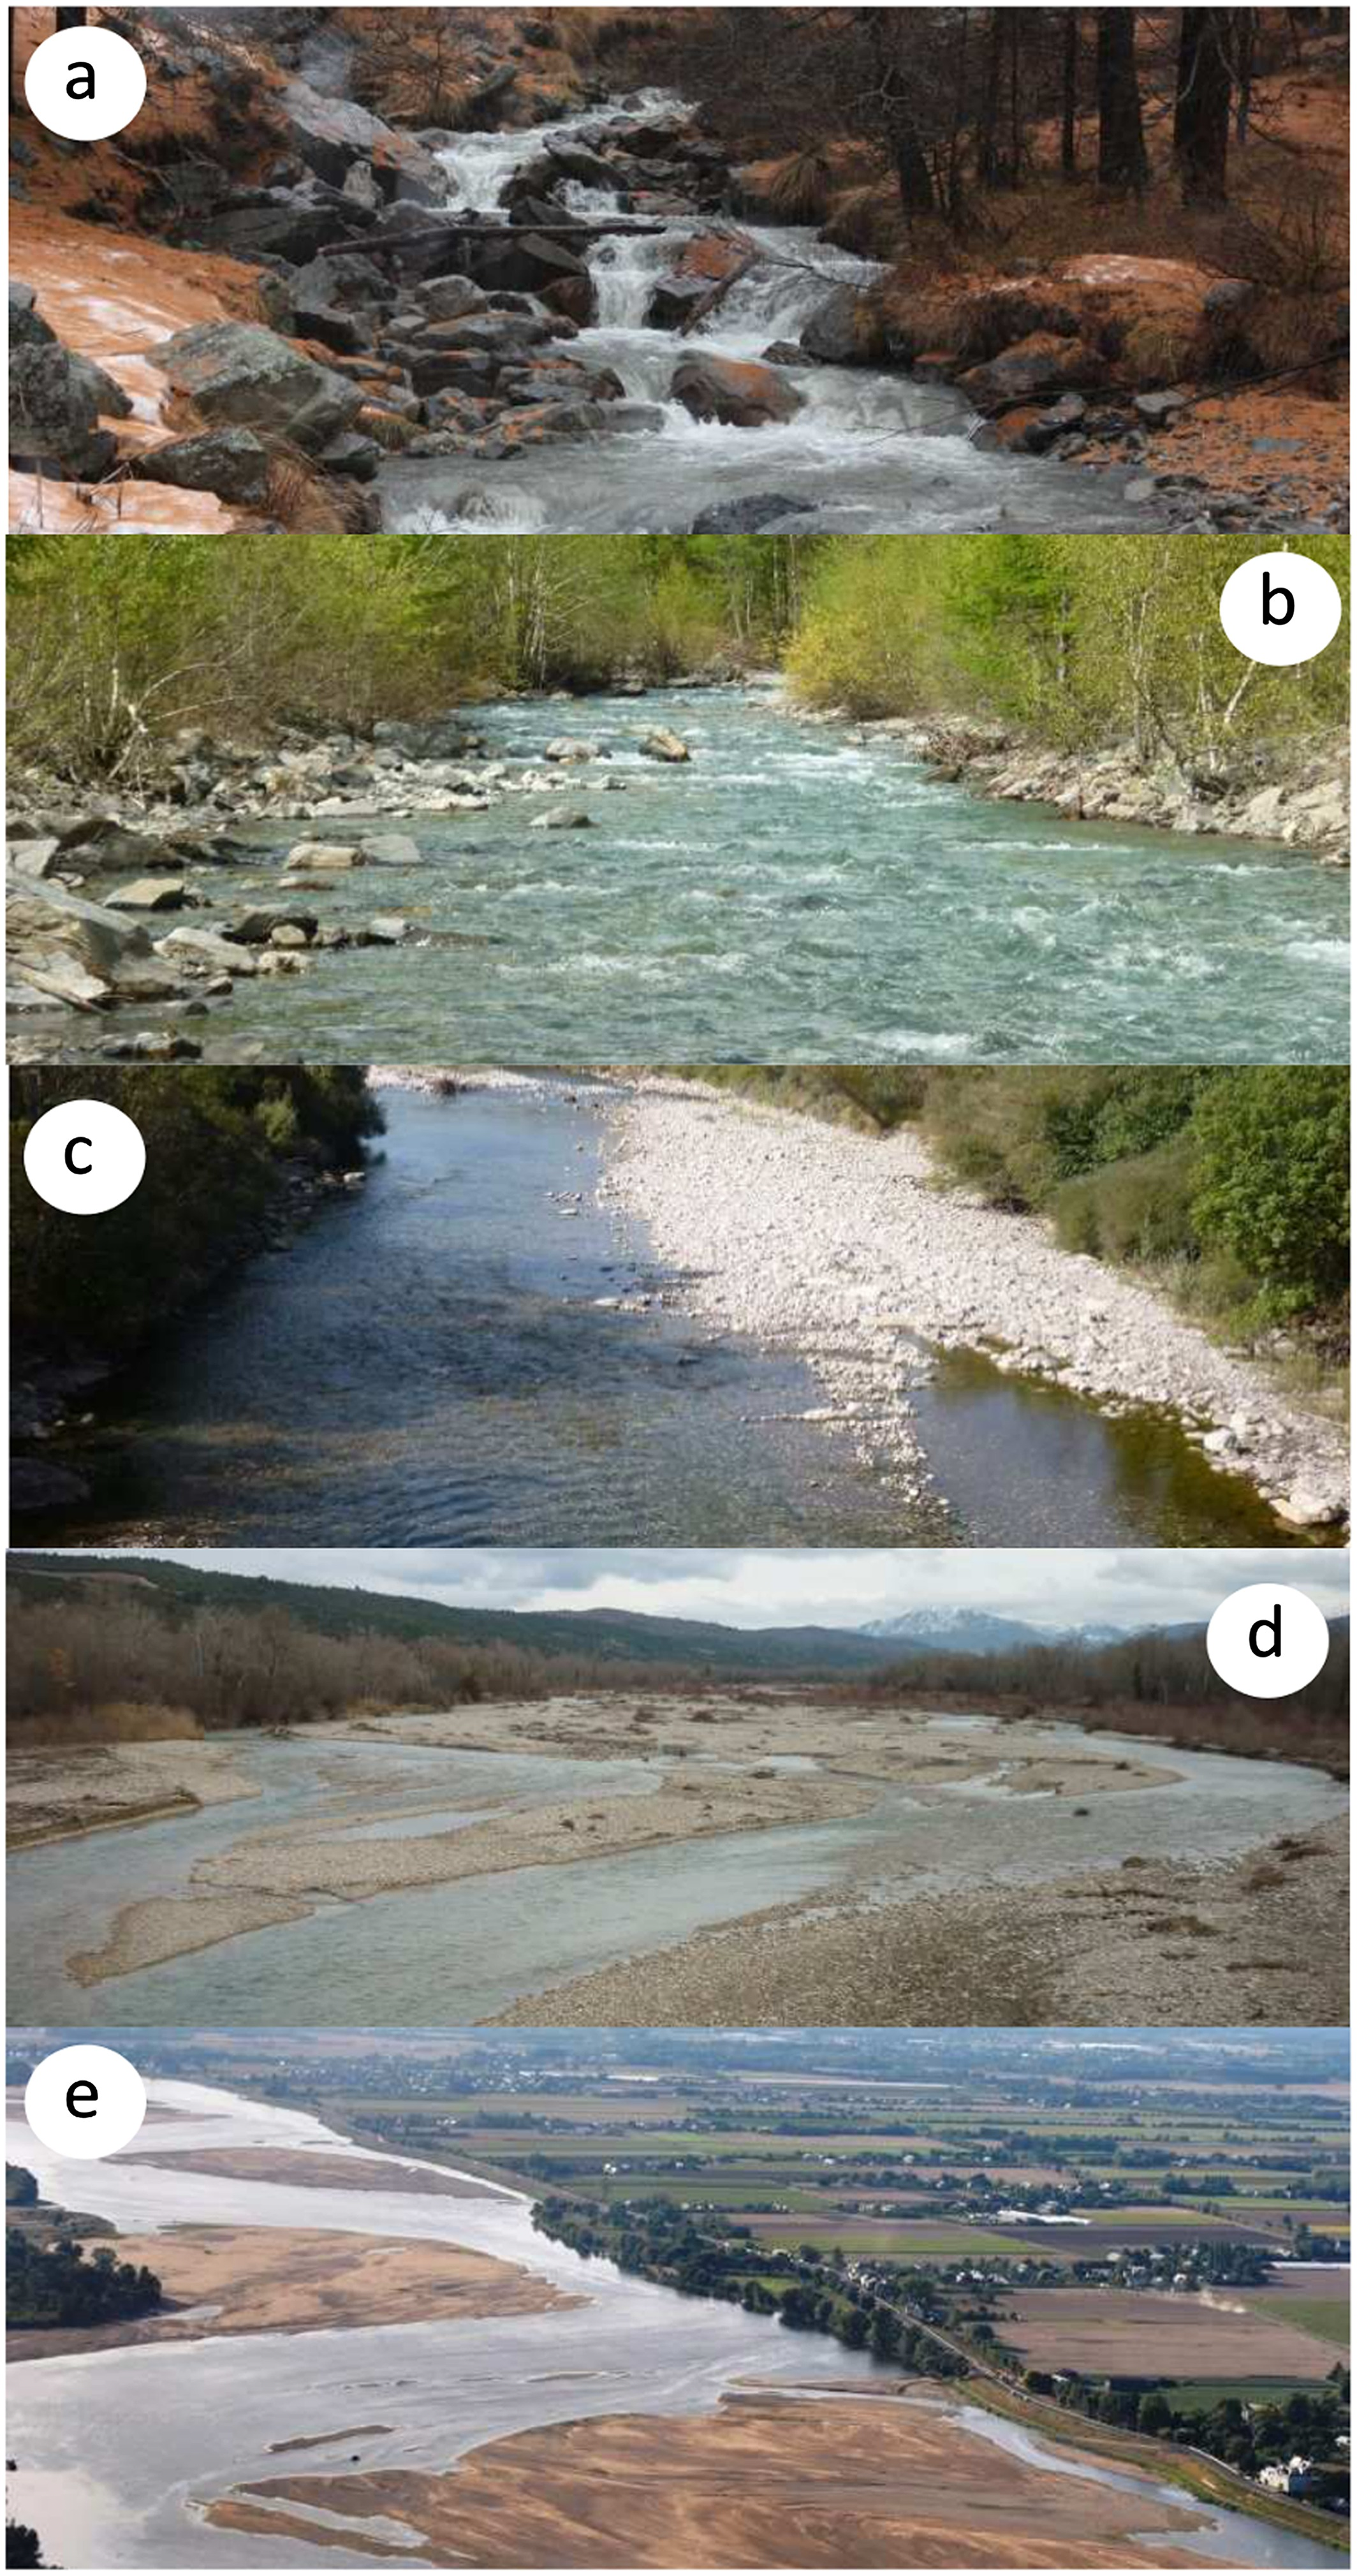
\includegraphics[width=0.45\textwidth]{./graphics/recking2015.jpg}
    \caption{(a) A step-pool stream (Tinée), (b) a plane-bed stream (Byasse), (c) a riffle-pool stream (Drac), (d) a braided stream (Bléone), (e) a sand-bed river (Loire). © S. Rodrigez. from Recking et al. \cite{recking2015}}
    \label{fig:morpho_recking2015}
\end{figure}

\newpage
%----------------------------------------------------------------------------------------
%	APPENDIX B: Examples of cas and xcas files
%----------------------------------------------------------------------------------------
\chapter{Examples of cas and xcas files}
\section{The \xcas}
\label{app:xcas}
\lstinputlisting[language=xml]{../../../examples/courlis/lefort/depot_lefort_sarap.xcas}

\section{The \cas}
\label{app:cas}
\subsection{\Cbedload example}
\lstinputlisting[language=TelemacCasRed]{../../../examples/courlis/lefort/depot_lefort_courlis_sarap.cas}
\subsection{\Csuspension example}
\lstinputlisting[language=TelemacCasRed]{../../../examples/courlis/Garonne/hydro_courlis.cas}
\newpage
%---------------------------------------------------------------------------
% Bibliography
%---------------------------------------------------------------------------

\bibliographystyle{plainnat}
%\bibliography{../../data/biblio}
\bibliography{./latex/courlis_user_guide.bib}
\end{document}
